% !TeX spellcheck = ru_RU
%pdflatex, utf8
\documentclass[unicode, 10pt, a5paper, oneside]{article}

% Установка полей страницы
%\usepackage{anysize}
%\marginsize{0.3cm}{0.3cm}{0.3cm}{0.3cm}
\usepackage[a5paper, margin=0.3cm, bindingoffset=0cm]{geometry}

% Поддержка русского языка
\usepackage[T2A]{fontenc}		% Корректная кодировка шрифта при использовании cm-super
\usepackage[utf8]{inputenc}		% Кодировка ввода
\usepackage[russian]{babel}		% Словарь расстановки переносов
%\usepackage{cmap}				% Перекодировка символов в pdf при использовании обычного cm

% Всякие математические фишки
\usepackage{amsmath}
\usepackage{amsfonts}
\usepackage{amssymb}

% Изменение цвета, работа с графикой
\usepackage{color}
\usepackage[pdftex]{graphicx}
\graphicspath{{images/}}

% Команда для вставки ссылок \url{URL}
\usepackage[hyphens]{url}
\urlstyle{rm}					% Стиль шрифта ссылок: с засечками

% Кликабельные ссылки внутри документа
\usepackage[unicode]{hyperref}

% Включает отступ у первого абзаца в разделе
\usepackage{indentfirst}

% Настрйока стиля списков
\usepackage{enumitem}
\setlist{noitemsep, leftmargin=*, labelindent=\parindent, topsep=0pt, parsep=0pt, partopsep=0pt}

\setlist[itemize,1]{label=$\diamond$}
\setlist[itemize,2]{label=\textendash}
\setlist[itemize,3]{label=$\star$}

\renewcommand{\alph}[1]{\asbuk{#1}} % Костыль для кирилической нумерации вместо латинской
\setlist[enumerate,1]{label=\arabic*)}
\setlist[enumerate,2]{label=\alph*)}
\setlist[enumerate,3]{label=(\arabic*)}


\usepackage{textcomp}			% Команды для вставки разных символов (градусы, проценты, итд)
\usepackage{float}				% Размещение плавающих объектов там где они созданы (X)
\usepackage{wrapfig}			% Обтекаемые текстом рисунки

% Подписи у флоатов
\setlength{\intextsep}{0pt} % Отстут вокруг плавающих окружений
\usepackage{caption}
\captionsetup{parskip=0pt}
\captionsetup[figure]{labelsep=period,justification=centering,singlelinecheck=false,textfont=small,labelfont=small,aboveskip=2pt,belowskip=0pt}

% Изменение формата заголовков разделов
\usepackage{titlesec}
\titleformat{\section}{\newpage\small\bfseries}{\thesection. }{0pt}{}{}
\titlespacing*{\section}{0pt}{0pt}{0pt}

\titleformat{\subsection}{\small\bfseries}{\thesubsection. }{0pt}{}{}
\titlespacing*{\subsection}{0pt}{0pt}{0pt}

\usepackage{array}				% Позволяет объявить свои типы колонок
\usepackage{calc}				% Математика, исп-ся для расчёта ширины колонки
\usepackage{longtable}			% Длинные таблицы

% Минимальный отступ в таблицах
\setlength{\tabcolsep}{1.5mm}

% Новые типы колонок. Ширина задётся как доля от linewidth
\newcolumntype{L}[1]{p{#1\linewidth-2\tabcolsep-2\arrayrulewidth}}
\newcolumntype{C}[1]{>{\centering}p{#1\linewidth-2\tabcolsep-2\arrayrulewidth}}
\newcolumntype{R}[1]{>{\raggedleft}p{#1\linewidth-2\tabcolsep-2\arrayrulewidth}}
\newcolumntype{U}[2]{p{#1\linewidth-(#2)}}

% Стараться не оставлять одиноких строк в начале и конце абзаца
\clubpenalty=1000
\widowpenalty=1000

% Расстановка отступов и переносов
\emergencystretch=2.5em			% Максимальный промежуток между словами
\tolerance=2000
\frenchspacing


\begin{document}

\setcounter{section}{60}

% Вопрос 61 -----------------------------------------------------------------
\section{Организация и этапы разработки конструкторских документов.}

Существуют следующие стадии разработки КД.
\begin{enumerate}
\item ТЗ устанавливает основное назначение, технические и тактико-технические характеристики, показатели качества и технико-экономические требования предъявляемые к разрабатываемому изделию, выполнение необходимых стадий разработки КД и ее состав, а также специальные требования к изделию.
\item Техническое предложение --- совокупность конструкторских документов, которые должны содержать техническое и технико-экономическое обоснование целесообразности разработки документации изделия на основании анализа технического задания заказчика и различных вариантов возможных решений изделия, сравнительной оценке решений с учетом конструктивных и эксплуатационных особенностей разрабатываемого и существующих изделий, а также патентных материалов.
\item Эскизный проект --- совокупность КД, которые должны содержать принципиальные конструктивные решения, дающие общее представление об устройстве и принципе работы изделия, а также данные, определяющие назначение, основные  параметры, габаритные размеры разрабатываемого изделия, 
\item Технический проект --- совокупность конструкторских документов, которые должны содержать окончательные технические решения, дающее полное представление об устройстве разрабатываемого изделия и исходные данные для разработки рабочей документации.
\item Разработка рабочей документации опытного образца с литерами “О1” и “О2” и др., установочной серии с литерой “А”, установившегося серийного или массового производства с литерой “Б”.
\end{enumerate}


% Вопрос 62 -----------------------------------------------------------------
\section{Виды КД.}

КД подразделяются:
\begin{enumerate}
\item на единичные;
\item групповые --- изделия, обладающие общими конструктивными признаками и имеющие некоторые отличия друг от друга.
\end{enumerate}

Графические:
\begin{enumerate}
\item чертеж детали --- изготовление детали и данные необходимые для ее изготовления, контроля и испытаний;
\item сборочный чертеж (СБ) --- изображение изделия и данные, необходимые для его сборки (изготовления) и контроля;
\item чертеж общего вида (ВО) --- изображение конструкции изделия, дающее представление о взаимодействии его основных частей и принципе работы. Выполняется на этапе эскизного проектирования;
\item теоретический чертеж (ТЧ) --- геометрическая форма изделия и координаты его основных частей;
\item габаритный чертеж (ГЧ) --- контурное (упрощенное) изображение изделия с габаритными, установочными и присоединительными размерами;
\item монтажный чертеж (МЧ) --- контурное (упрощенное) изображение изделия, содержащее данные для его установки(монтажа);
\item схема --- условные изображения или обозначения составных частей изделия и связей между ними;
\item спецификация --- состав сборочной единицы комплекса или комплекта.
\end{enumerate}

Текстовые:
\begin{itemize}
\item ведомость спецификации (ВС) --- перечень всех спецификаций составных частей изделия с указанием из количества и входимости;
\item  ведомость ссылочных документов (ВД) --- перечень ссылочных документов, на которые имеются ссылки в КД;
\item ведомость покупных частей (ВП) --- перечень покупных изделий, примененных в составе разрабатываемого изделия; \item ведомость согласования применения покупных изделий (ВИ) --- подтверждение согласования с соответствующими организациями применения определенных покупных изделий в разрабатываемом изделии;
\item ведомость держателей подлинников (ДП) --- перечня предприятий, на которых хранятся подлинники документов, разработанных для данного изделия;
\item ведомость технического предложения (ПТ), эскизного (ЭП), технического (ТП) проекта --- перечень документов, вошедших в техническое предложение (ЭП, ТП);
\item пояснительная записка (ПЗ) --- описание устройства и принципа действия разработанного изделия, а также обоснование принятых при его разработке технико-экономических решений;
\item технические условия (ТУ) --- потребительские (эксплутационные) показатели изделия и методы контроля его качества;
\item программа и методика испытаний (ПМ) --- технические данные, подлежащие проверке при испытании изделия, а также порядок и методы их контроля;
\item таблица (ТБ) --- номенклатура таблиц, содержащих данные;
\item документы прочие (Д) --- все документы, которых нет в стандартах ЕСКД;
\item расчет (РР) --- расчет параметров и величин, например, расчет размерных (РР) цепи, электрических режимов и т.д.; \item эксплуатационные документы --- предназначены для использования при эксплуатации, обслуживании, ремонте и в процессе эксплуатации;
\item ремонтные документы (РД) --- служащие для проведения ремонтных работ на специализированных предприятиях;
\item инструкция (И) --- указания и правила, используемые при изготовлении изделия (сборке, регулировке, контроле и т.п.);
\item патентный формуляр (ПФ) --- содержит сведения о патентной чистоте объекта, а также о созданных и используемых при его разработке отечественных изобретениях;
\item карта технического уровня и качества изделия (КУ) --- содержит данные, определяющие технический уровень качества изделий и соответствие его технических и экономических показателей достижениям науки и техники, а также потребностям народного хозяйства.
\end{itemize}

Наименование КД в зависимости от способа их выполнения:
\begin{enumerate}
\item оригиналы --- документ,  выполненный на  любом материале и предназначенный для изготовления по ним подлинников;
\item подлинники --- документ, оформленный подлинными установленными подписями и выполненные на любом материале, позволяющим многократное воспроизведение с них копий;
\item дубликаты --- копии с подлинников; 
\item копии --- документы, выполненные способом, обеспечивающим их идентичность с подлинником.
\end{enumerate}


% Вопрос 63 -----------------------------------------------------------------
\section{Стандартизация и БНК.}

Стандартизация --- это установление и применение правил с целью упорядочения деятельности в определенной области.

Задачи стандартизации: разработка требований к качеству готовых изделий на основе комплексной стандартизации их характеристик; установление требований и методов в области проектирования и производства РЭА; введение единых систем документации; установление единых требований и обозначений.

Составные части стандартизации: типизация; агрегатирование; унификация.

Типизация --- это способ ликвидации излишнего многообразия изделий путем их обоснованного сведения к ограниченному числу избранных типов (типоразмеров), при котором размеры и параметры изменяются с определенным шагом.

Унификация подразумевает создание типовых (модульных) конструкций, размеры сторон которых изменяются по метрическому или ритмическому соотношениям, прилагаемых ко всем или некоторым габаритным размерам. При метрическом соотношении значения n-го размера составляют:
\begin{equation}
a_n=a_0+n \cdot m
\end{equation}
При ритмическом $a_n=a_0*K_m$, где $a_0$ --- начальное значение размера; n --- целое или дробное число, лежащее в основе целого размерного параметрического ряда; m --- величина приращения при метрическом соотношении; $K_m$ --- коэффициент прогрессии ритмического соотношения.
БНК. 

Несущая конструкция(НК) --- это элемент или совокупность конструктивных элементов, предназначенных для размещения составных частей изделия, обеспечения их конструктивной целостности и неизменности в соответствии с конструкторской документацией. НК, имеющая стандартизированные размеры и конструктивное решение, обязательное при конструировании радиоэлектронных средств различного функционального значения, называется базовой несущей конструкцией (БНК). БНК имеют три структурных уровня:
\begin{itemize}
\item  БНК1 (ячейка, кассета и др.) --- для размещения электронных модулей нулевого уровня, изделий электронной техники и электротехнических изделий;
\item БНК2 (блок, вставной блок, блочный каркас и др.) --- для размещения радиоэлектронного средства, выполненного на основе БНК1;
\item БНК3 (шкаф, стойка, стеллаж, рама, пульт оператора, приборный стол и др.) --- для размещения радиоэлектронного средства, выполненного на основе БНК2 и (или) БНК1.Вся сложная ЭА в настоящее время строится на основе каких-либо БНК (принципы модульности, стандартизации, унификации, отсюда следует совместимость и взаимозаменяемость электронных модулей). При использовании БНК конструирование ЭА сводится к разработке новых печатных плат внутри- и меж- блочного монтажа и передних панелей.
\end{itemize}

Существуют каркасные и бескаркасные БНК, у первых стойкость, прочность, жесткость и устойчивость конструкции обеспечивается наличием каркаса, у вторых --- совокупностью других составляющих его элементов.

Элементы несущих конструкций ЭС предназначены для размещения и крепления компонентов электрической части изделия, передачи и распределения температурных нагрузок, защиты от механических воздействий и др. факторов внешней среды.
    
Анализируя структурные уровни ЭС можно выделить соответствующие им структурные уровни базовых несущих конструкций (табл. 5.4).
%table
\begin{center}\small
\begin{tabular}{|c|c|c|}
\hline Обозначения структурного& &\\ уровня & ЭС & БНК \\  
\hline 0 & ЭРЭ, ИС, БИС & Подложка, корпус \\  &(покупные изделия) & \\
\hline 1 & Объемные модули, микромодули, МСБ & Плата\\
\hline 2 & Функциональные узлы & Плата в сборе\\
\hline 3 & Блок & Каркас(корпус)\\
\hline 4 & Конструктивно и функционально & Стойка, шкаф, \\ & законченое изделие &  стеллаж, рама\\
\hline
\end{tabular}
\end{center}

 Кроме указанных БНК, при конструировании ЭС всех структурных уровней применяют другие элементы несущих конструкций: профили, основания, направляющие, кожухи, обшивки, основания, рамки, панели, экраны, воздуховоды, радиаторы, элементы фиксации, элементы крепления и др.
 
Выбор материалов и правила конструирования печатных плат достаточно известны из литературы и частично были рассмотрены нами ранее. Остальные элементы несущих конструкций, как правило, выполняются из металлов и сплавов и выполняют роль элементов жесткости общей конструкции. В некоторых случаях они несут силовую нагрузку и поэтому должны быть рассчитаны согласно основным формулам теории прочности и упругих деформаций.

система «ЕС-902» --- разработана на основе стандартов DIN и международной эл. технической комиссии (МЭК) и включает в себя два основных типоразмера ПП --- «С» и «F» и два соответствующих им типоразмера комплексных корпусов; система «INTERMAS» --- современная универсальная вариантная конструкторская система, отвечающая требованиям высокой плотности монтажа, рационального производства и автоматизированной сборки и эл. монтажа. Применяется как в серийном производстве, так и при индивидуальном. Более развита структура, чем у ES --- 902. Для  INTERMAS и ES --- 902 2,54 мм единый размерный модуль; 

“НАДЕЛ-85”- система, служащая для построения электронных измерительных приборов или соответствующих им по сложности РЭС, работающих как при стационарном размещении, так и в подвижном (закрытые кузова автомобилей, закрытые помещения судов).

Состав системы “Надел-85” показан на рисунке. система «Надел-82» --- позволяет в короткие сроки формировать как подвижные, так и стационарные измерительные системы, системы с телеметрическими каналами связи. Система работает в технологических комплексах, специальных измерительных системах. По своим размерам и ТТ соответствует ГОСТу 26765.17 --- 90.
\begin{figure}[H]
\centering
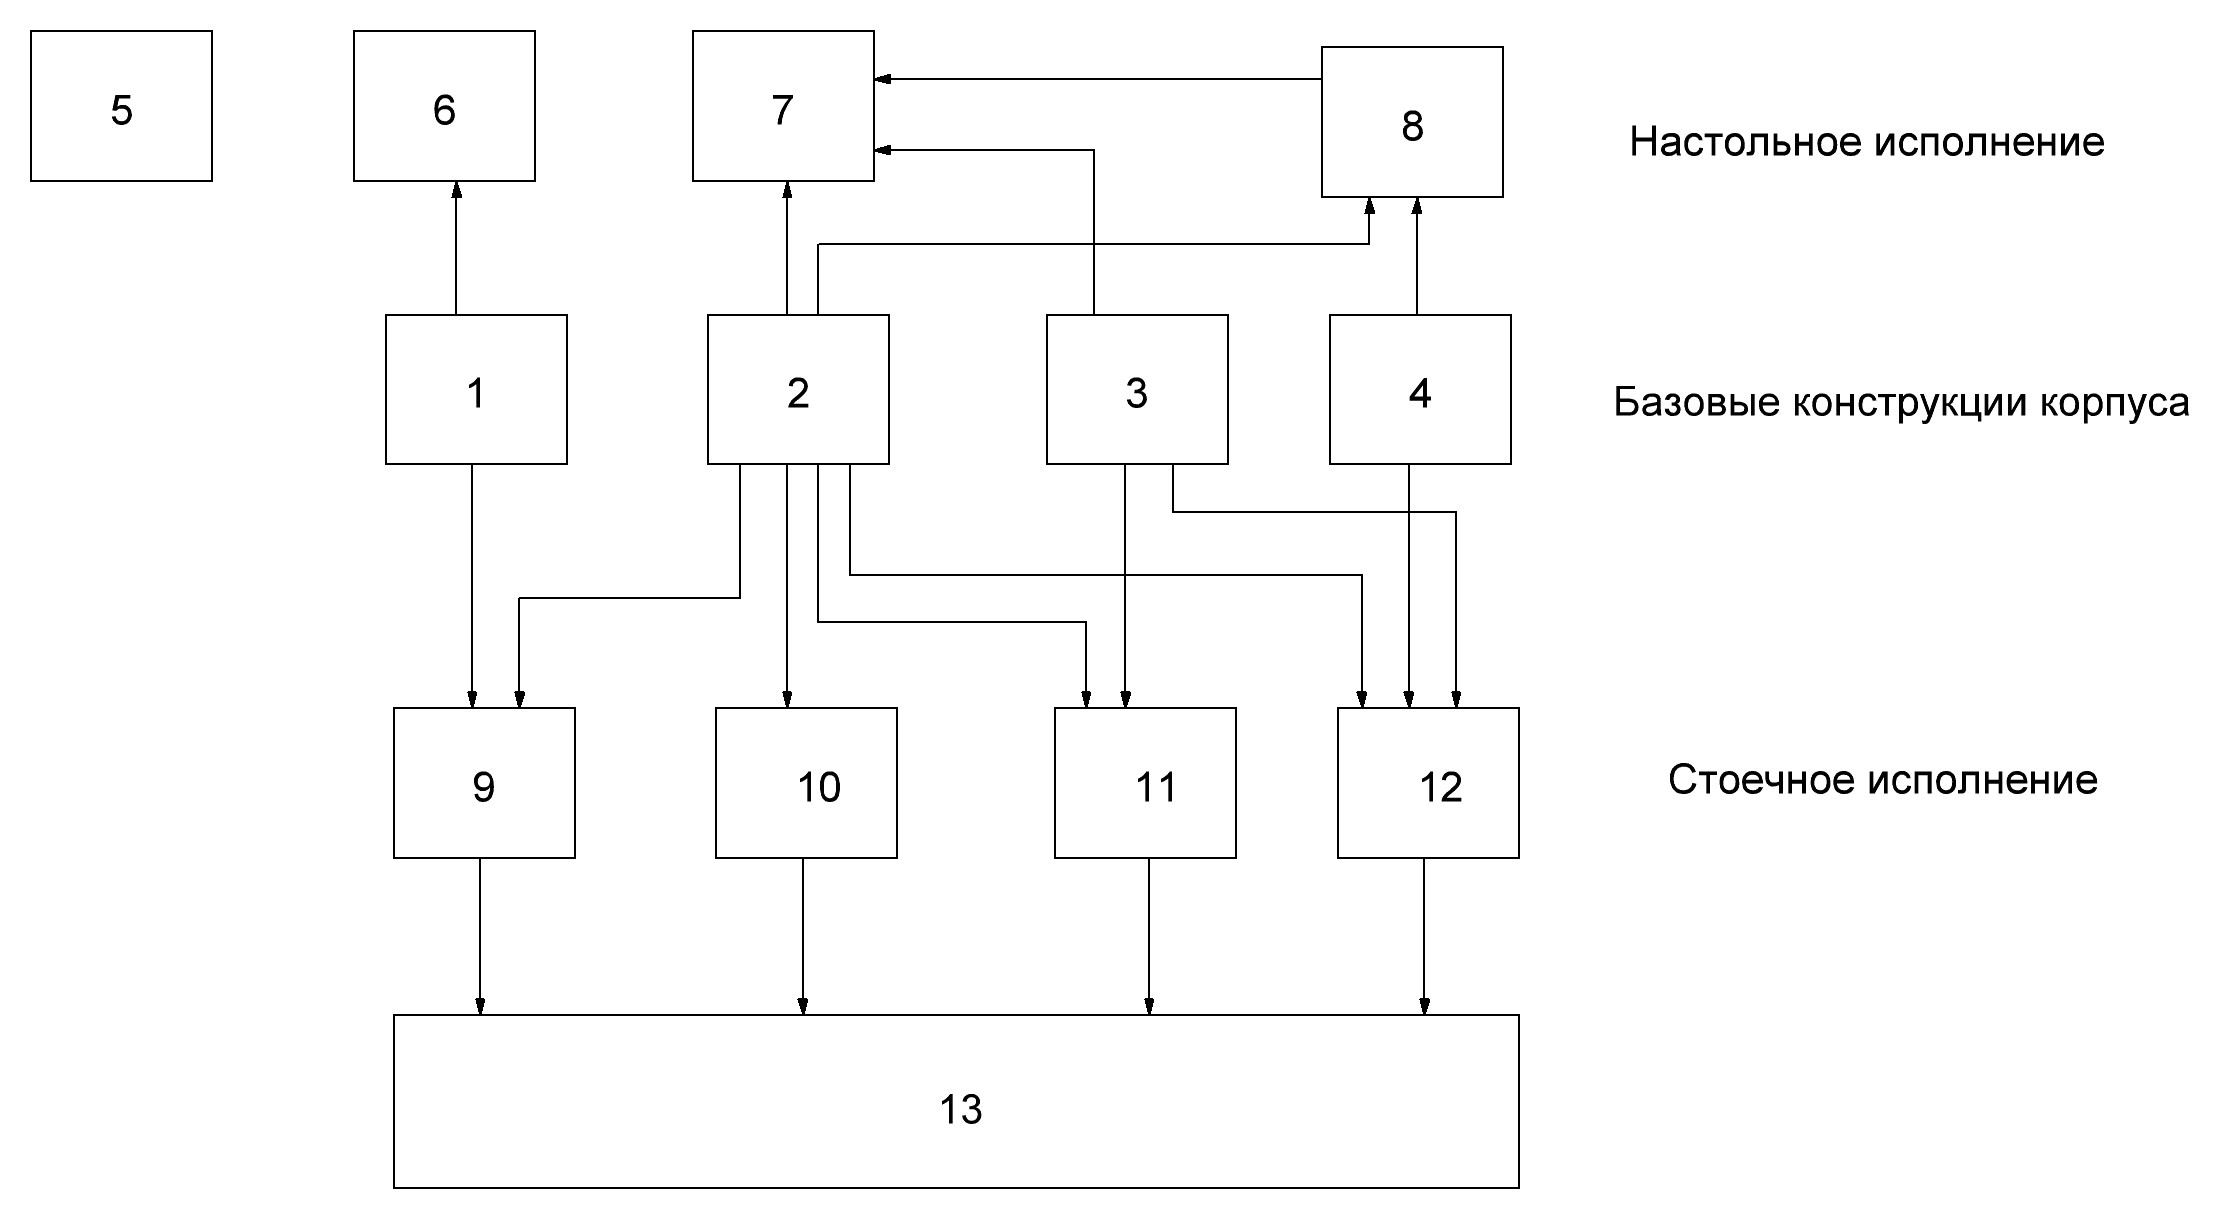
\includegraphics[width=0.8\textwidth]{63_Sistema.JPG}
\caption{Конструкционная система электронных приборов}
\end{figure}
\begin{center}
\begin{enumerate}
\item малогабаритный агрегатируемый корпус;
\item настольно-стоечный корпус;
\item вставной блок;
\item малогабаритный осцилографический корпус;
\item малогабаритный неагрегатируемый корпус;
\item настольно-переносной корпус;
\item агрегатирование настольно-переносных корпусов по вертикали;
\item варианты конструкций настольных осциллографических блоков;
\item агрегатирование по ширине; 
\item стоечное исполнение базового корпуса;
\item установка вставных блоков и осциллографа;
\item стоечный вариант конструкции с рамой;
\item установка стоечных блоков в шкаф.
\end{enumerate}
\end{center}


% Вопрос 64 -----------------------------------------------------------------
\section{Виды и типы схем, обозначения по ЕСКД.}
\underline{Виды схем}:
\begin{itemize}
\item электрические (Э);
\item  гидравлические (Г);
\item  пневматические (П);
\item  газовые (Х); 
\item кинематические (К);
\item  вакуумные (В); 
\item оптические (Л);
\item энергетические (Р);
\item  деления (Е);
\item  комбинированные (С).
\end{itemize}

\underline{Типы схем:}
\begin{enumerate}
\item структурные (1) --- отображает принцип работы изделия в общем виде. На схеме изображают все основные функциональные части изделия, а также основные взаимосвязи между ними. Действительное расположение составных частей изделия не учитывают и способ связи не раскрывают. Построение схемы должно давать наглядное представление о последовательности взаимодействия функциональных частей в изделии. Направление хода процессов, происходящих в изделии, обозначают стрелками на линиях взаимосвязи. Функциональные части на схеме изображают в виде прямоугольников или условных графических обозначений. При обозначении функциональных частей в виде прямоугольников их наименования, типы, и обозначения вписывают внутрь прямоугольников;
\item функциональные (2) --- на схеме изображают функциональные части изделия (элементы, устройства и функциональные группы) и связи между ними. Графическое построение схемы должно наглядно отражать последовательность функциональных процессов, иллюстрируемых схемой. Действительное расположение в изделии элементов и устройств может не учитываться. Функциональные части и связи между ними изображают в виде УГО. Отдельные функциональные части на схеме допускается изображать в виде прямоугольников;
\item принципиальные (3) --- является наиболее полной электрической схемой изделия, на которой изображают все электрические элементы устройства, необходимые для осуществления и контроля в изделии заданных электрических процессов, все связи между ними, а также элементы подключения (разъемы, зажимы), которыми заканчиваются входные и выходные цепи. На схеме могут быть изображены соединительные и монтажные элементы, устанавливаемые в изделии по конструктивным соображениям;
\item соединений (монтажные) (4) --- определяет конструктивное выполнение электрических соединений элементов в изделии. На схеме изображают все устройства и элементы, входящие в состав изделия, их входные и выходные элементы (соединители, платы, зажимы и т.п.) и соединения между ними. Устройства изображают в виде прямоугольников или упрощенных внешних очертаний, элементы --- в виде условных графических обозначений, установленных в стандартах ЕСКД, прямоугольников или упрощенных внешних очертаний;
\item подключения (5) --- показывает внешние подключения изделия. На схеме должны быть изображены изделие, его входные и выходные элементы (соединители, зажимы и т.п.) и подводимые к ним концы проводов и кабелей внешнего монтажа, около которых помещают данные о подключении изделия (хар-ки внешних цепей, адреса) На схеме изделия и их составные части изображают в виде прямоугольников, а входные и выходные элементы (соединители) --- в виде условных графических обозначений;
\item общие (6) --- на схеме изображают устройства и элементы, входящие в комплекс, а также соединяющие их провода, жгуты и кабели Устройства и элементы изображают в виде прямоугольников;
\item расположения (7) --- определяет относительное расположение составных частей изделия, а при необходимости, также жгутов, проводов, кабелей. На схеме изображают составные части изделия и при необходимости связи между ними, а также конструкцию, помещение или местность, на которых эти части расположены. Составные части изделия изображают в виде упрощенных внешних очертаний или УГО, которые располагают в соответствии с действительным размещением частей изделия в конструкции или на местности. Провода, жгуты и кабели изображают в виде отдельных линий или упрощенных внешних очертаний;
\item объединенные (0).
\end{enumerate}


% Вопрос 65 -----------------------------------------------------------------
\section{Методы компоновки конструкции ЭВС.}

Каждый из методов применяется на том или ином этапе разработки аппаратуры, имеет свои особенности выполнения и оформления компоновочных элементов, в зависимости от выбранной элементной базы, способа монтажа соединений и компоновочного уровня:
\begin{itemize}
\item Аналитическая компоновка --- проводится на ранних стадиях разработки ЭВА и представляет собой прикидочную оценку основных компоновочных характеристик РЭА, блока, узла. Для изделий малой сложности или малого блока производится расчёт:

\begin{eqnarray}
\centering
V_{\Sigma}=\frac{1}{k_{v}}\left(\sum^{n}V_{\sigma_{i}}+\sum^{m}V_{a_{i}}\right)
\end{eqnarray}
Где $V_{\Sigma}$---общий объем изделия
$k_{v}$---обобщенный коэффициент заполнения объема изделиями;
$V_{\sigma_{i}}$ и $V_{a_{i}}$---значения установочных объемов однотипных и единичных элементов
\begin{eqnarray}
\centering
G=K_{G}\sum^{n}G_{i}
\end{eqnarray}
Где $G$---масса аппарата;
$K_{G}$---обобщенный коэффициент объемной массы изделия;
\begin{eqnarray}
\centering
G=G'V_{\Sigma}
\end{eqnarray}
Где $G'$---объемная масса аппарата.

Для изделий большой сложности, расчет компоновочных характеристик проводится по укрупнённым характеристикам.
\item Номографическая компоновка --- является частным видом аналитической компоновки и для расчета основных показателей компоновки исполь-я номограммы оцифрованные в условных единицах установочных объёмов. Эта компоновка также исполь-я на этапе ТП, для из-й малой сложности 
Преимущества:

\begin{enumerate} 
\item повышенная точность расчёта (10…15 \%); 
\item значительно ниже трудоёмкость (< 1 часа). 
\end{enumerate}

\item Аппликационная компоновка --- в отличие от рассмотренных выше имеет наглядность. Сущность в том, что на тонком картоне, плотной бумаге вычерчивают необходимые проекции компонентов изделия. Вычерчивают в масштабе 2:1, 5:1 и более или 1:1, 1:2, 1:5. После вычерчивания аппликацию вырезают по контуру.
\item Модельная компоновка --- при изготовлении объёмных моделей элементов, формы их выбирают такими, чтобы они имели простые но характерные обводы. Клееные модели из плотной бумаги или тонкого картона могут быть только простых форм (цилиндры, конусы, кубы и т.п.). Модели крепят с помощью профилированных отв-й, шпилек, гаек. Мелкие модели выполняют из пластилина. 
\item Графическая компоновка --- при этом используют упрощённые способы начертания элементов. Существуют чертежи элементов с различной степенью детализации их начертания:
\begin{enumerate} 
\item изображения дающие подробные сведения о геометрической форме деталей;
\item  контурные --- дают полное представление о форме детали;
\item  условное изображение детали в виде прямоугольников. Большое удобство даёт использование специальных трафаретов из целлулоида или органического стекла, в котором выполнены контуры деталей. Удобно использовать цветное изображение. Соединительные линии выполняют наклейкой или вычерчиванием.
\end{enumerate}
 
\item Натурная компоновка --- при этом вместо моделей или аппликаций пользуются реальными элементами. Три способа натурной компоновки:
\begin{enumerate}
\item собирают все Эл-ы уст-ва, плотно укладывают их в коробку и задаваясь коэф заполнения объёма, пересчитывают полученное значение объёма;
\item элементы подготавливают к монтажу и раскладывают их в необходимом порядке на листе бумаги, затем место расположения элементов обозначают простым карандашом, а места пайки цветным. Наложив лист пергамента по цветным точкам выполняют монтажный эскиз;
\item используя элементы уст-ва, выполняют его макет.
\end{enumerate}
\item Машинная компоновка --- является одной из стадий машинного проектирования РЭА. Из-за высокого уровня унификации конструктивных элементов их машинное проектирование является наиболее распространённым.
\end{itemize}


% Вопрос 66 -----------------------------------------------------------------
\section{Климатические зоны и категории исполнения.}

Климат --- характерная для данной области на поверхности Земли совокупность типичных изменений атмосферных процессов, обусловливаемых географическими координатами, уровнем солнечной радиации, строением земной поверхности и т.д.
\begin{center}\small
\begin{tabular}{|c|c|}
\hline Категории& Характеристика\\исполнения & места \\  изделий & размещения\\
\hline 1 & на открытом воздухе \\ 
\hline 2 & Под навесом или открытых помещениях \\
\hline 3 & В закрытых помещениях с естественной вентиляцией\\ & без искусственного регулирования климатических условий \\
\hline 4 & В помещениях с искусственным регулированием климатических условий\\
\hline 5 & В помещениях с повышенной влажностью \\
\hline
\end{tabular}
\end{center}

Климатическое исполнение электротехнических изделий.
\begin{center}
\begin{tabular}{|c|c|}
\hline Климатическое& Характеристика климата\\исполнения &  \\ 
\hline У & Умеренный (t = -45..40 \textcelsius) \\ 
\hline УХЛ & Умеренный и холодный \\
\hline ХЛ & Холодный (-45 \textcelsius )\\ 
\hline ТВ & Тропический влажный (t $\geqslant$ 20 \textcelsius , влажн $\geqslant$ 80 \%)\\
\hline ТС & Тропический сухой (t $\geqslant$ 40 \textcelsius) \\
\hline T & Тропический (как сухой так и влажный)\\
\hline O & Любой климат на суше, кроме очень холодного\\
\hline M & Морской \\
\hline TM & Тропический морской \\
\hline OM & Любой морской климат \\
\hline B & Всеклиматический \\
\hline
\end{tabular}
\end{center}

Условия эксплуатации РЭА:
\begin{itemize}
\item Нормальные (t=25\textpm 100\textcelsius, г=45…80\%, Р=630…800 мм.рт.ст.);
\item Легкие (t=20\textcelsius, г<80 \%, P $\approx$ 760 мм.рт.ст.). нет воздействия пыли, песка, излучения и биологической среды. Характерно для закрытых, отапливаемых и вентилируемых помещений;
\item средние (t=-50…+70\textcelsius, r<98\%) воздействие пыли, песка, биологической среды. Характерно для наземной, полевой и передвижной аппаратуры.
\item жесткие (t=-80…+100\textcelsius, r<90\%, $P<5 \cdot 10^-6$ Па.) воздействие пыли, песка, фонового излучения среднего уровня. Характерно для авиационной РЭА.
\item особо жесткие (t=-100…+250\textcelsius, r<90\%, $P<5 \cdot 10^-6$ Па) воздействие сильных фоновых излучений, пыли.
\end{itemize}

% Вопрос 67 -----------------------------------------------------------------
\section{Способы защиты ЭВС от влаги.}

Частичная герметизация --- ей подвергаются наименее стойкие к внешним воздействиям детали и узлы. При этом кожух не является герметизирующим элементом. Основной метод --- изолирование жидкими диэлектриками.

Полная герметизация --- достигается применением защитных корпусов из металла, керамики и др.

Комбинированная герметизация --- используются защитные корпуса, компаунды, изолирующие плёнки, лаки и др.

Консервация --- защита от коррозии наружных поверхностей с помощью пушечной смазки или технического вазелина.

Пропитка --- заполнение пор, трещин, пустот в изоляционных материалах, а также промежутков между конструктивными элементами узлов электроизоляционными негигроскопическими материалами.

Заливка --- заполнение диэлектриком свободного промежутка между заливаемым изделием и стенками кожуха.

Обволакивание --- процесс покрытия изделия плёнкой. Применяют эмали и покровные лаки. Кроме этого применяют влагостойкие материалы (стёкла, керамика, слюда, кварц); высоколегированные нержавеющие сплавы (Х18Н9Т, Х18Н10Т, бронзы БрБ2 и титановые сплавы ВТ-0), легированные сплавы (Х13, 1Х13); применяют антикоррозионные покрытия (никелирование, цинкование, кадмирование). ПП покрывают двумя, тремя слоями лака (УР-231, Э-4100, СБ-1С). Для высокотемпературных узлов применяют кремнийорганические лаки (К-57, К-47). Изделия из металла для тропического исполнения покрывают эмалями (ЭП-51, ПФ-163).

\textit{Примеры конструкций средств защиты}

Схемы герметичных соединений конструктивных элементов металлических корпусов: 
\begin{itemize}
\item соединение пайкой
\begin{figure}[H]
\centering
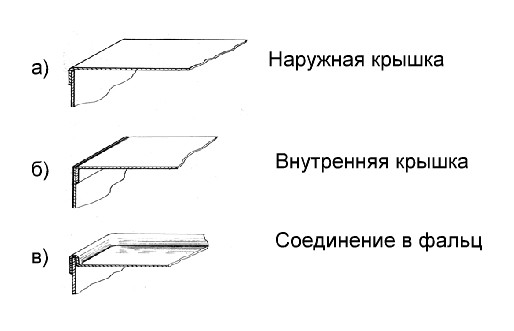
\includegraphics[width=0.6\textwidth]{67_paiko.JPG}
\caption{виды соединения пайкой}
\end{figure}

\item соединение дуговой сваркой
\begin{figure}[H]
\centering
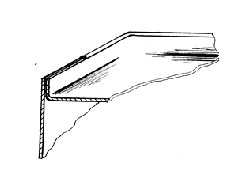
\includegraphics[width=0.3\textwidth]{67_dug_svar.JPG}
\caption{соединение дуговой сваркой}
\end{figure}
\item соединение контактной сваркой
\begin{figure}[H]
\centering
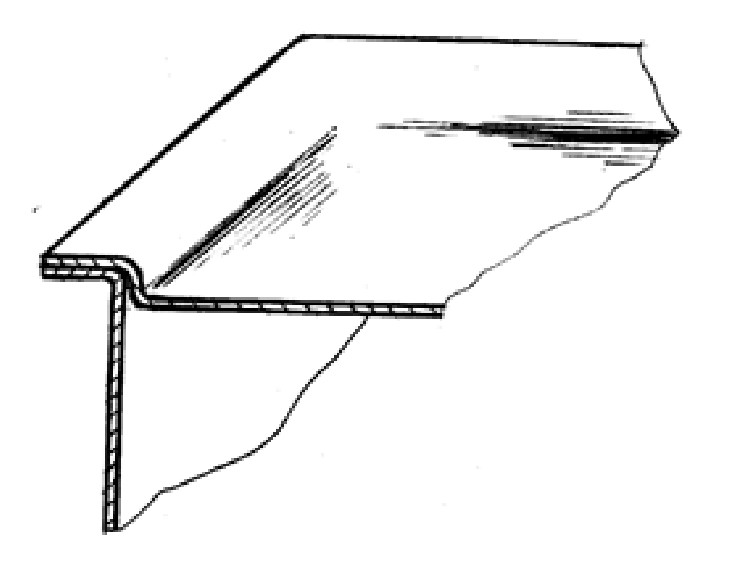
\includegraphics[width=0.3\textwidth]{67_kont_svar.JPG}
\caption{соединение контактной сваркой}
\end{figure}
\item герметизация при помощи резиновых прокладок
\begin{figure}[H]
\centering
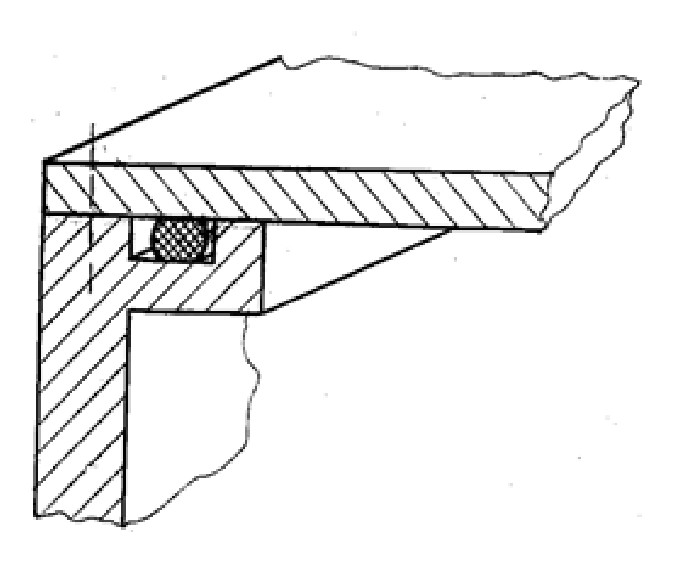
\includegraphics[width=0.3\textwidth]{67_prokladka.JPG}
\caption{герметизация резиновой прокладкой}
\end{figure}
\end{itemize}

Уплотнение герметизированной РЭА с помощью фетрового  и фторопластового сальника.
\begin{figure}[H]
\centering
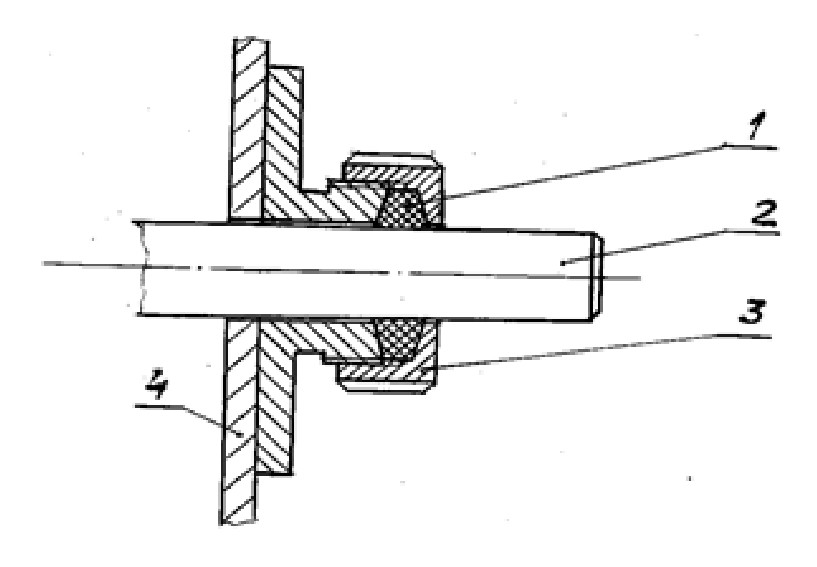
\includegraphics[width=0.3\textwidth]{67_fetr.JPG}
\caption{1- фетровый сальник; 2- валик; 3- накладная гайка; 4- корпус.}
\end{figure}


% Вопрос 68 -----------------------------------------------------------------
\section{Защита ЭВС от механических воздействий.}

При эксплуатации и транспортировке на МЭА, действуют вибрации, удары и линейные ускорения. Так, например, вибрации характеризуется перегрузками, достигающими 30g в диапазоне частот от 30 до 5000 Гц, а линейные ускорения и удары --- перегрузками до 50g. Действие этих факторов может привести к поломке выводов, подложек микросхем, возникновению в них усталостных напряжений, разрушению контактов и герметизации блоков.

Защита ЭВС осуществляется следующими группами методов:  Уменьшение интенсивности источников механического воздействия (путем их балансировки, уменьшение зазоров, виброизоляция самого источника механических воздействий); Уменьшение величины передаваемых ЭВС воздействий (путем его виброизоляции, демпфирования, устранения резонансов, активной виброзащиты с помощью эксцентриков, маятников, гироскопов); Используются наиболее прочные и жесткие компоненты и узлы.

Принцип виброизоляции заключается в размещение между объектом установки и ЭВС специальных устройств --- амортизаторов, которые поглощают и отражают механическую энергию. Поглощение энергии колебаний происходит демпфированием за счет трения в материале амортизаторов или в демпферах с сухим или вязким трением между элементами конструкции. Эффективность виброизоляции ($\gamma$) равным отношению амплитуды возмущающих колебаний к амплитуде вынужденных колебаний амортизирующего ЭВС.

Амортизаторы:
\begin{enumerate}
\item Металлорезиновая (АП, АКСС-М, АКСС-И, АО и др.);
\item Металлопружинные (АПН, ДК, АТ и др.).
\end{enumerate}
Основные типы амортизаторов (нормализованные):
\begin{enumerate}
\item Амортизатор демпфированный
\begin{figure}[H]
\centering
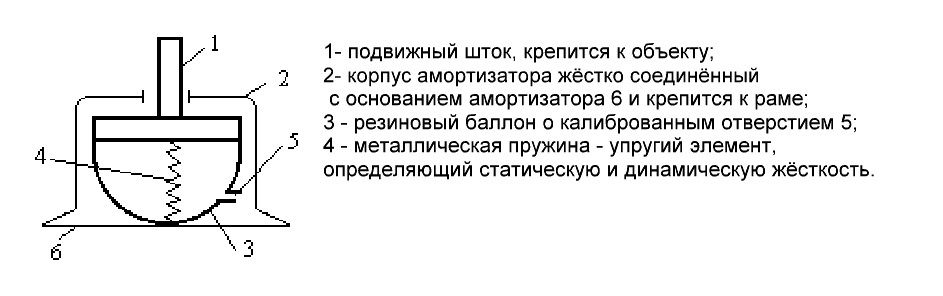
\includegraphics[width=0.8\textwidth]{68_AD2.JPG}
\caption{Амортизатор демпфированный}
\end{figure}
При вибрационных нагрузках баллон деформируется и через калиброванное отверстие проходит воздух внутрь и в баллон, следовательно происходит рассеивание энергии, т.о. осуществляется демпфирование.
недостатки этого амортизатора:
\begin{itemize}
\item	наличие резиновой детали --- старение, боится солнечной радиации. 
\item	невозможность эксплуатации при большой разреженности атмосферы (непригоден для самолётов, ракет, высокогорий.).
\end{itemize}

\item Амортизатор фрикционного демпфирования
\begin{figure}[H]
\centering
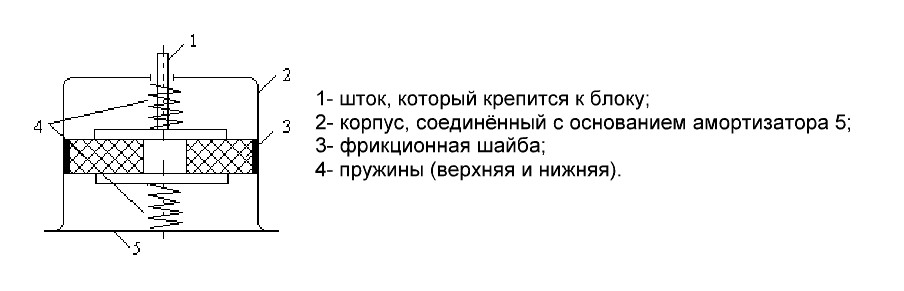
\includegraphics[width=0.8\textwidth]{68_AFD.JPG}
\caption{Амортизатор фрикционно демпфированный}
\end{figure}

Этот амортизатор лишён недостатков амортизаторов 1-го типа.

\item амортизатор пространственного нагружения
\begin{figure}[H]
\centering
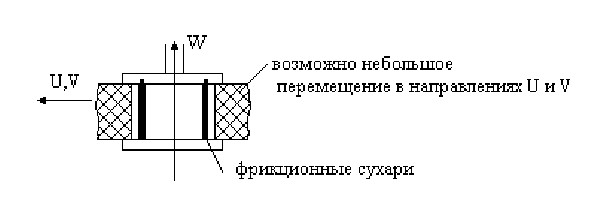
\includegraphics[width=0.8\textwidth]{68_APN.JPG}
\caption{Амортизатор пространственного нагружения}
\end{figure}

Дополнительные диссипативные силы образуются за счёт трения шайбы о сухари, следовательно, возможны нагрузки не только в направлении W.
\item Амортизатор плоскостный (или чашечный)

\begin{figure}[H]
\centering
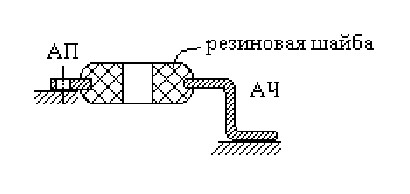
\includegraphics[width=0.5\textwidth]{68_AP.JPG}
\caption{Амортизатор плоскостный}
\end{figure}

Резиновая шайба  определяет упругие силы и упругие свойства амортизатора.

Основные параметры этого амортизатора совпадают с параметрами амортизаторов типа АД, кроме  требований разрежения.
Жесткость и прочность обеспечиваются ребрами жесткости, отбортовкой, заливкой, обволакиванием.

\end{enumerate}

\underline{Рекомендации по защите РЭА от вибрационных воздействий} \nopagebreak
\begin{enumerate}
\item	Уменьшение внешних вибрационных воздействий возможно только при амортизации блока. При этом параметры вибрации блока могут быть снижены на 1..2 порядка по сравнению с возмущающим воздействием.
\item Устанавливать блок без амортизаторов целесообразно при действии вибрации в течении 10…20\% времени от общего времени эксплуатации устройства.
\item	Амортизаторы целесообразно ставить в том случае, если РЭА регулярно подвергается вибрационным воздействиям (подвижная, бортовая, корабельная).
\end{enumerate}

% Вопрос 69 -----------------------------------------------------------------
\section{Способы обеспечения теплового режима ЭВС.}

Имеется много систем охлаждения, и они характеризуются рядом факторов. По способу поглощения тепла различают системы на основе фазовых переходов (испарение, плавление) веществ, и термоэлектрического эффекта и термоаккумуляционные системы. Теплоносителями могут служить газы, жидкости, твердые тела. В системах применяют естественное и искусственное охлаждение.

К естественному охлаждению относятся системы, где охлаждение происходит наружной средой поверхности аппарата или естественно-испарительными фитильными устройствами (тепловыми трубками). Естественное воздушное охлаждение является наиболее простым, надежным и дешевым способом, однако он используется при небольших удельных мощностях.  Естественное воздушное охлаждение широко используется не только для общего охлаждения, но и для охлаждения отдельных тепловыделяющих элементов. Повышение эффективности достигается путем увеличения теплопроводящей поверхности с помощью радиаторов.

Принудительное охлаждение осуществляется продувкой внутренней зоны прибора воздухом, наружным обдувом его поверхности, перемешиванием воздуха внутри аппарата, использованием микрохолодильных и термостатирующих устройств, жидких и воздушных испарительных систем и за счет термоаккумуляционных свойств материала.

Принудительная вентиляция подразделяется на приточную, вытяжную и приточно-вытяжную. Наиболее эффективным является жидкостно-испарительные системы, где охлаждение производиться за счет циркуляции охлаждающей жидкости. Воздушно-испарительные устройства работают на основе испаряемых жидкостей с низкой температурой кипения.
 
При компоновке блоков МЭА с целью обеспечения нормального теплового режима существуют некоторые общие рекомендации, а именно:
\begin{itemize}
\item более нагретые ячейки и субблоки следует монтировать ближе к основанию-теплоотводу блока,
\item для уменьшения локальных перегревов отдельные термочувствительные узлы необходимо выносить на корпус или в ниши блока, а более мощные ИС и транзисторы следует располагать по периферии ячейки, ближе к рамке, 
\item блоки питания желательно разбивать на несколько отдельных субблоков (трансформаторных, стабилизаторных и т. п.) для увеличения суммарной поверхности теплоотдачи,
\item при наличии внешнего обдува целесообразно оребрение корпусов, причем ребра должны располагаться вдоль потока воздуха.
\end{itemize}


% Вопрос 70 -----------------------------------------------------------------
\section{Электромагнитные воздействия. Виды экранов.}

При прохождении мощных сигналов по цепям связи последние становятся источниками электромагнитных полей, которые пересекают другие цепи связи. Могут наводить в них существенные дополнительные помехи. Источниками электромагнитных помех являются мощные промышленные установки, двигатели, различные коммуникации. Устройства чувствительные к электрическим, магнитным, статическим полям могут неустойчиво работать. Поэтому для устранения этого воздействия используют экранирование.

Экранирование --- это локализация электромагнитной энергии в определенном пространстве конструкционными методами.

Составляющие экранирования: экраны, стаканы, промежуточные стенки корпуса, оплетка ПМЛ на проводах, кабель РК, фильтры.

\subsection*{Виды экранов}

\begin{enumerate}
\item Металлический лист.

Физический смысл экранирующего эффекта, получаемого от металлического листа, соединенного с корпусом прибора, заключается в создании короткого замыкания на корпус для большей части паразитной емкости, имеющейся между экранируемыми друг друга точками.

Эффективность экранирования электрического поля  определяется исключительно отношением паразитных емкостей между точками А и Б до и после установки экранирующего листа. Любые мероприятия, приводящие к снижению, увеличивают эффективность экранирования.

\begin{figure}[H]
\centering
\hspace{0.15\textwidth}
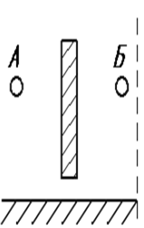
\includegraphics[width=0.1\linewidth]{70_met_list.png}
\hspace{0.1\textwidth}
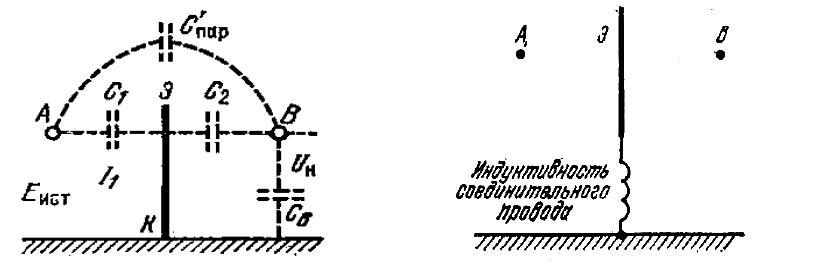
\includegraphics[width=0.6\linewidth]{70_met_eq.png}\\
a) \hspace{0.4\textwidth} б) \hspace{0.1\textwidth}
\caption{Металлический экран (а), экран соединённый с корпусом (б)}
\end{figure}


\item Экран из ферромагнитного материала с большой магнитной проницаемостью (метод шунтирования экраном).

Метод шунтирования магнитного поля экраном применяется для защиты от постоянного и медленно изменяющего переменного магнитного поля. Экраны изготавливаются из ферромагнитных материалов с большой относительной магнитной проницательностью (сталь, пермаллой). При наличии экрана линии магнитной индукции проходят в основном по его стенкам, которые обладают малым магнитным сопротивлением по сравнению с воздушным пространством внутри экрана.  Качество экранирования зависит от магнитной проницаемости экрана и сопротивления магнитопровода, т.е. чем толще экран и чем меньше швов, стыков, идущих поперек направления линий магнитной индукции, эффективность экранирования будет выше.

\begin{figure}[H]
\centering
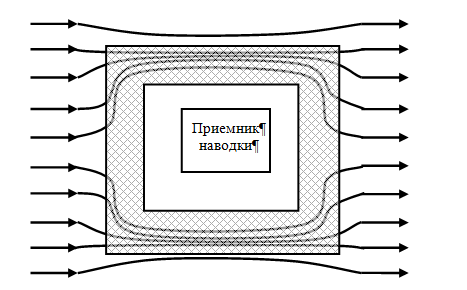
\includegraphics[width=0.5\linewidth]{70_ferro.png}
\caption{Экран из ферромагнитного материала}
\end{figure}


\item Метод вытеснения магнитного поля экраном.

Метод вытеснения магнитного поля экраном применяется для экранирования переменных высокочастотных магнитных полей. При этом используются экраны из немагнитных металлов. Экранирование основано на явлении индукции. Здесь явление индукции полезно.

Поставим на пути равномерного переменного магнитного поля (а) медный цилиндр. В нем возбудятся переменные ЭД, которые, в свою очередь, создадут переменные индукционные вихревые токи (токи Фуко). Магнитное поле этих токов (б) будет замкнутым; внутри цилиндра оно будет направлено навстречу возбуждающему полю, а за его пределами --- в ту же сторону, что и возбуждающее поле. Результирующее поле (в) оказывается ослабленным у цилиндра и усиленным вне его, т.е. происходит вытеснение поля из пространства, занимаемого цилиндром, в чем и заключается его экранирующее действие, которое будет тем эффективнее, чем меньше электрическое сопротивление цилиндра, т.е. чем больше протекающие по нему вихревые токи.

\begin{figure}[H]
\centering
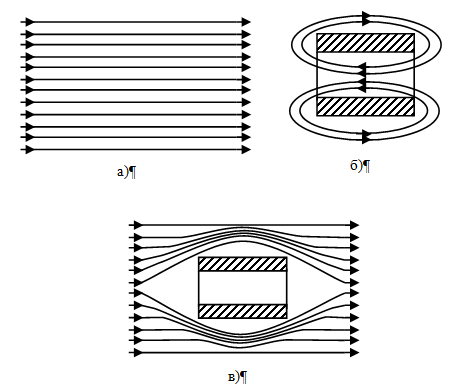
\includegraphics[width=0.5\linewidth]{70_vytesn.png}
\caption{Вытеснение магнитного поля вихревыми токами}
\end{figure}
\end{enumerate}


% Вопрос 71 -----------------------------------------------------------------
\section{Виды линий связи.}

Линии связи бывают электрически длинными, если время распространения сигнала больше фронта импульса: «длинные» соединения делают в виде согласованных экранированных линий связи.

Исключение: задержка сигнала, уменьшение амплитуды сигнала. Большинство соединений можно отнести к электрически «коротким». Линия связи считается электрически короткой, если длительность фронта импульса больше времени задержки распространения сигнала(4Тз).

Исключение: ухудшение фронтов, появление паразитных сигналов на плоской части импульса.

Основные искажающие факторы --- эффект отражений и различного рода помехи.

\subsection*{Различные конструктивные виды линий связи.}

В ЭС особенно старших конструктивных уровней (стойки) могут сочетаться различные типы линий (связь двух элементов, расположенных на различных несущих конструкциях) может включать следующие участки:

\texttt{Микрополосковая линия -- контакт -- разъемы -- витая пара -- контакт -- разъем -- микрополосковая линия.}

Степень искажения сигнала зависит от электрических параметров топологии и геометрические длины различных соединений.

Помехи, возникшие при конструктивной реализации межсхемных соединений не должны превышать допустимых, а задержки сигналов должны обеспечивать определенные в ТЗ быстродействие.

\subsection*{Электрические параметры линий связи}

\begin{wrapfigure}{o}{0.4\textwidth}
\centering
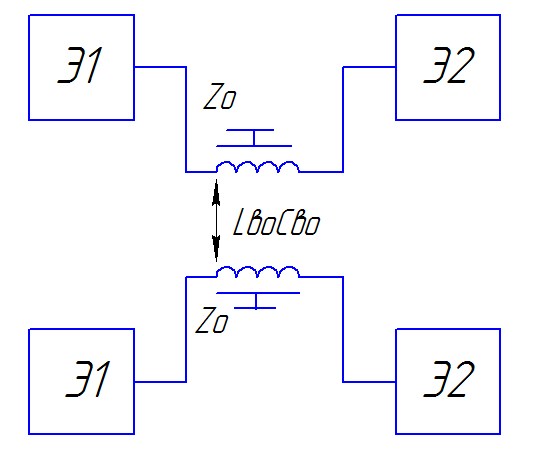
\includegraphics[width=0.7\linewidth]{71_raspred.png}
\caption{Схема взаимодействия цепей связи с распределенными параметрами}
\end{wrapfigure}

На рисунке $ L_\text{вo} $, $ C_\text{вo} $ --- взаимные емкость и индуктивность на единицу длины линии; $ Z_0 $ --- волновое сопротивление линии.

\begin{equation}
Z_0 = \dfrac{\sqrt{R_0 + j\omega L_0}}{G_0 + j \omega C_0}\text{, где}
\end{equation}
\par $ R_0, G_0 $ --- активное сопротивление линии и проводников изоляции на единицу длины линии;
\par $ C_0, L_0 $ --- собственная емкость и индуктивность, т.к. $ R_0, G_0 $ малы.

Ниже приведены некоторые виды связи, применяемые в ЭС и формулы для расчета их основных электрических параметров.

Здесь и далее $ h $ и $ d $ --- в мм; $ C_0 $ --- Ф/м;   $ L_0 $ --- в Гн/м; $ Z_0 $ --- в Ом.
% Тут ещё был какой-то непонятно к чему относящийся капитанский рисунок...

\begin{enumerate}
\item Витая пара.\nopagebreak

\begin{minipage}{\linewidth}
	\begin{wrapfigure}{o}{0.4\linewidth}
	\centering
	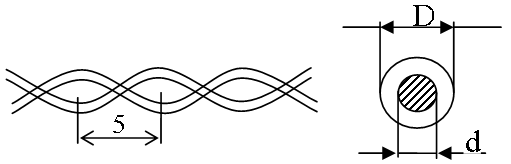
\includegraphics[width=0.9\linewidth]{71_vit_pair.png}
	\caption{Витая пара}
	\end{wrapfigure}
	
	\begin{equation}
	L_0 = 2 \cdot 10^{-7} \ln \dfrac{2D}{d}.
	\end{equation}

	\begin{equation}
	C_0 = \dfrac{120}{\sqrt{\varepsilon_\text{эфф}}} \ln \dfrac{2D}{d}.
	\end{equation}
\end{minipage}
\vspace{1em}

\item Полосковая линия.\nopagebreak

\begin{minipage}{\linewidth}
	\begin{wrapfigure}{o}{0.4\textwidth}
	\centering
	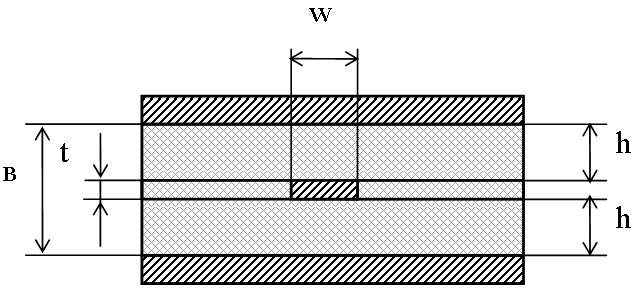
\includegraphics[width=\linewidth]{71_polos_line.png}
	\caption{Полосковая линия}
	\end{wrapfigure}
	
	\begin{equation}
	C_0 = 0,355 \cdot 10^{-10} \dfrac{\varepsilon_\text{эфф} W}{b (1 - t/n)}.
	\end{equation}

	\begin{equation}
	L_0 = \dfrac{1,38}{3 \cdot 10^6} \log \dfrac{16 h}{\pi w}.
	\end{equation}
	
	Если $ \dfrac{w}{b} \geq 0,35 $:
	
	\begin{equation}
	Z_0 = \dfrac{60}{\sqrt{\varepsilon_\text{эфф}}} \ln \dfrac{4b}{0,576w + 0,67t}.
	\end{equation}
	
	Если $ \dfrac{w}{b} \leq 0,35 $:
	
	\begin{equation}
	Z_0 = \dfrac{60}{\sqrt{\varepsilon_\text{эфф}}} \ln \dfrac{4b}{0,67\pi (0,8w + t)}.
	\end{equation}
\end{minipage}
\vspace{1em}

\item Микрополосковая линия.\nopagebreak

\begin{minipage}{\linewidth}
	\begin{wrapfigure}{o}{0.4\linewidth}
	\centering
	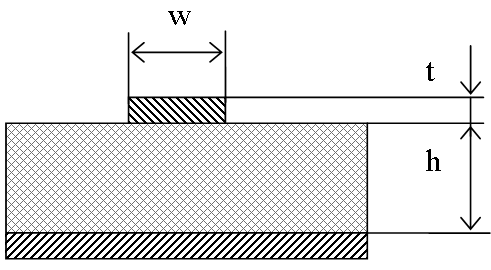
\includegraphics[width=0.9\linewidth]{71_micropolos_line.png}
	\caption{Микрополосковая линия}
	\end{wrapfigure}
	
	\begin{equation}
	C_0 = 0,355 \cdot 10^{-9} \dfrac{w}{4\pi h}.
	\end{equation}

	\begin{equation}
	L_0 = 3,77 \dfrac{\mu h}{3 \cdot 10^6 w}.
	\end{equation}
	
	\begin{equation}
	Z_0 = \dfrac{87}{\sqrt{\varepsilon_\text{эфф} + 1,41}} \ln \dfrac{5,98 h}{0,8w + t}.
	\end{equation}
\end{minipage}
\vspace{1em}

\item Коаксиальный кабель.\nopagebreak

\begin{minipage}{\linewidth}
	\begin{wrapfigure}{o}{0.4\linewidth}
	\centering
	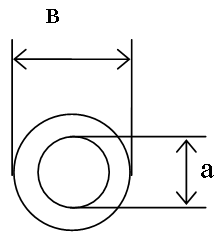
\includegraphics[width=0.4\linewidth]{71_koaksial.png}
	\caption{Коаксиальный кабель}
	\end{wrapfigure}
	
	\begin{equation}
	L_0 = \dfrac{138\mu}{3 \cdot 10^8} \log\dfrac{b}{a}.
	\end{equation}\vspace{\parsep}

	\begin{equation}
	C_0 = 2\pi \dfrac{\varepsilon_\text{эфф}}{\ln(b/a)}.
	\end{equation}
\end{minipage}
\vspace{1em}

\end{enumerate}


% Вопрос 72 -----------------------------------------------------------------
\section{Особенности конструирования бортовых ЭВС.}

Бортовые РЭС отличаются большим разнообразием применения по назначению: связь, радиолокационные станции, бортовые ЭВМ и т.д. Условия работы авиационной, ракетной и космической РЭА характеризуется пониженным значением атмосферного давления. В таблице приведена зависимость рабочих значений атм.давления от высоты над уровнем моря.

\begin{center}
\begin{tabular}{|l|c|c|c|c|c|c|c|c|c|c|c|}
\hline
H, км		& 1		& 2		& 3		& 4		& 6		& 8		& 10	& 12	& 18	& 26	& 31	\\ \hline
P, мм.рт.ст	& 674	& 596	& 526	& 462	& 354	& 267	& 199	& 145	& 57	& 16	& 7,7	\\ \hline
\end{tabular}
\end{center}

Влияние пониженного давления на работоспособность РЭА проявляется через явления:
\begin{enumerate}
\item Уменьшается электрическая прочность воздушного пространства;
\item Ухудшается конвекция, что вызывает дополнительный перегрев изделий.
\end{enumerate}

Зависимость коэффициента относительной электрической прочности ($ K_Z $) воздушных промежутков от высоты над уровнем моря приведена в таблице.
\begin{center}
\begin{tabular}{|l|c|c|c|c|c|c|c|c|c|c|c|c|c|c|}
\hline
H ,км 	& 1 & 2		& 3		& 4		& 6		& 8		& 10	& 12	& 14	& 16	& 18	& --	& 26	& 31	\\ \hline
$ K_Z $ & 1 & 0,9	& 0,8	& 0,72	& 0,56	& 0,45	& 0,35	& 0,3	& 0,25	& 0,19	& 0,14	& 0,1	& 0,05	& 0,03	\\ \hline
\end{tabular}
\end{center}

С уменьшением давления (ниже 6-7 мм.рт.ст.), т.е. с увеличением высоты (>30-40км) электрическая прочность возрастает и подчиняется закону Пашена. Уменьшение конвективной теплопередачи определяется из рис. \ref{fig:72_graphs}, где $ k $ --- это отношение коэффициента теплопередачи при заданном и нормальных давлениях. Уменьшение теплоотдачи приводит к уменьшению электрической прочности из-за увеличения температуры деталей и узлов и окружающей их среды. Электрическая прочность зависит также и от функциональной $ f $, где $ U_f $ --- пробивное напряжение при $ f $.

\begin{figure}[H]
\centering
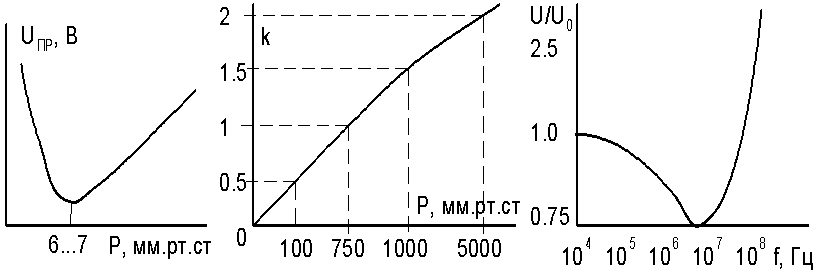
\includegraphics[width=0.8\linewidth]{72_graphs.png}
\caption{Изменение параметров с ростом высоты}\label{fig:72_graphs}
\end{figure}


% Вопрос 73 -----------------------------------------------------------------
\section{Особенности конструкций персональных ЭВМ.}

Основу конструкций любых ПЭВМ составляют печатные узлы с ИМС, ЭРЭ и другими элементами. В зависимости от количества используемых печатных узлов различают одноплатные и многоплатные конструкции. Одноплатные конструкции обычно содержат функционально всю схему компьютера. По такому варианту конструктивно реализуются, например, портативные и другие простейшие ПЭВМ.

В отличие от одноплатных, конструкции многоплатных ПЭВМ компонуются из нескольких печатных узлов, где центральная плата содержит схему минимальной конфигурации, остальные же функции системы реализуются на дополнительных платах. По такой схеме компонуются, например, профессиональные ПЭВМ.

Рассмотрим особенности конструкций настольных профессиональных ПЭВМ.

Обычно центральные и периферийные устройства профессиональных ПЭВМ, образующие конкретную вычислительную систему (системный блок, клавиатура, видеомонитор, печатающее устройство и др.), выполняются в виде самостоятельных независимых конструктивов --- модулей, которые можно удобно располагать на рабочем месте пользователя и соединять друг с другом электрическими кабелями.

Как правило, все функциональные устройства системного блока (процессор, память, устройства ввода-вывода и др.) реализуют в виде конструктивно законченных сборочных единиц (узлов) --- электронных модулей (ячеек), связь между которыми осуществляется по системной шине или с помощью кабелей.

Основу конструкции системного блока ПЭВМ составляет набор электронных модулей, механически и электрически соединенных между собой. Наиболее типичной является компоновка системного блока, когда он объединяет как электронные модули (процессора, оперативной памяти, адаптеров обязательных периферийных устройств), так и системы электропитания и охлаждения, громкоговоритель, а также разъемные соединители для подключения периферийных устройств. В большинстве современных ПЭВМ в системный блок встраиваются накопители на гибких и жестких магнитных или оптических дисках (дисководы), имеется также возможность установки некоторого количества дополнительных электронных модулей для расширения системы (например, дополнительной оперативной памяти, модулей профессиональной ориентации, коммуникационных адаптеров) или подключения специального блока расширения.

Электронные модули ПЭВМ конструктивно представляют собой монтажные печатные платы определенного типоразмера, обычно многослойные, на которых размещаются ИМС различной степени интеграции, в том числе микропроцессорные БИС и БИС системной поддержки, другие ЭРЭ, а также разъемные соединители. Эти элементы, размещаемые на плате, представляют собой электронное оборудование одной или нескольких функционально законченных частей ПЭВМ, например центрального процессора, оперативной памяти, адаптеров периферийных устройств и т. д.

Интерфейс электронных модулей, их внешняя электрическая коммутация в систему осуществляется с помощью разъемных соединителей. Как правило, используются разъемные соединители прямого сочленения, но могут применяться также и разъемы косвенного сочленения.

По архитектурно-конструктивному исполнению различают «закрытые» и «открытые» ПЭВМ. «Закрытая» ПЭВМ представляет, собой вычислительную систему, функции которой жестко установлены с помощью аппаратных средств при сборке на заводе-изготовителе. Пользователь такой ПЭВМ практически не может заменить модули на более совершенные или добавить в вычислительную систему дополнительные модули, например, расширить оперативную памяти или подключить адаптеры новых периферийных устройств. По «закрытому» принципу реализуются в основном портативные и наиболее простые (игровые, домашние) ПЭВМ.

Современные модели ПЭВМ обычно реализуются в виде открытой, модульной (развиваемой в функциональном отношении), системы. Поэтому «открытые» ПЭВМ получили наибольшее распространение. Дополнительные функции в вычислительной системе (расширение системы) реализуются подключением к системной шине добавочных электронных модулей. В этом случае пользователь может приобретать и устанавливать в своей ПЭВМ различные дополнительные сменные модули, выполненные обычно в виде съемных плат, позволяющие расширять возможности ПЭВМ за счет применения новых периферийных устройств, подключения ПЭВМ к другим ЭВМ или сетям. Такие ПЭВМ легко модернизируются, морально устаревшие электронные модули заменяются новыми, выполненными по более совершенной технологии.

Для механического и электрического соединения электронных модулей в системном блоке обычно используется объединительная коммутационная плата (панель), часто называемая «материнской». Именно этот сборочный узел содержит ответные части разъемных соединителей электронных модулей, образующих системную шину. Каждый «дочерний» модуль вставляется в разъемный соединитель объединительной платы и обеспечивает выполнение одной или большего числа специфичных электронных функций, необходимых для функционирования всей ПЭВМ. От способа соединения модулей, используемых типов и количества разъемных соединителей зависят стоимость ПЭВМ, ее эффективность, гибкость и ремонтопригодность.

Для защиты от внешних воздействий и электромагнитных помех основные компоненты системного блока помещают в корпус. Корпуса системных блоков, как правило, содержат минимальное количество деталей, доступны для сборки и разборки простейшими инструментами и приспособлениями. Базовой несущей конструкцией обычно является металлическое основание (поддон), на котором размещаются блок электронных модулей, блок питания, кронштейны для закрепления дисководов, громкоговорителя и некоторые другие конструктивные элементы. В состав корпуса, кроме основания, входят также металлический кожух, передняя (лицевая) и задняя панели (стенки).

В последние годы при конструктивной реализации системных блоков ПЭВМ часто используется принцип установки корпуса на ребро (типа «башня»), широко применяемый ранее в конструкциях мини-ЭВМ. Системная плата в этом случае размещается вертикально. Такой корпус позволяет размещать большее число дисководов (до 8 и более) и экономить место при размещении ПЭВМ на рабочем столе. Электрические соединения системного блока и периферийных устройств ПЭВМ осуществляются гибкими ленточными или специальными экранированными кабелями, которые заземляются на металлическом основании системного блока. Кабели от периферийных устройств сходятся в системный блок, где подключаются непосредственно к электронным модулям (адаптерам) через разъемные соединители косвенного сочленения. Широко используются также разъемы, в которых соединение с ленточными кабелями осуществляется прорезанием изоляции кабеля хвостовиками выводов и их контактированием с жилами кабелей.

\begin{figure}[H]
\centering
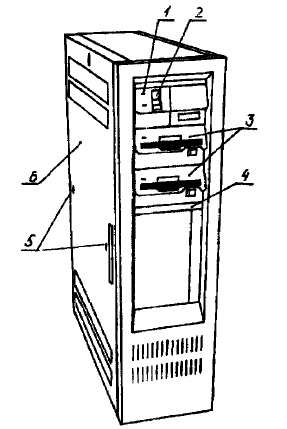
\includegraphics[width=0.25\linewidth]{73_tower.png}
\caption{Корпус типа <<башня>>}
\end{figure}



% Вопрос 74 -----------------------------------------------------------------
\section{Унификация. Разновидности стандартизации.}

\textit{Унификация} есть форма типизации конструкции, при которой размеры и параметры избранных типов, полученных путем деления или умножения на целые числа размеров и параметров одного исходного, базового.

Унификация подразумевает создание типовых (модульных) конструкций, размеры сторон которых могут изменяться по метрическому или ритмическому соотношениям, прилагаемым ко всем или только некоторым габаритным размерам. 

При метрическом соотношении значения n-го размера составляют: $ a_n=a_0+n_m $. При ритмическом $ a_n=a_0*K^{n}_{m} $, где $ a_0 $ --- начальное значение размера; $ n $ --- целое или дробное число, лежащее в основе целого размерного параметрического ряда; $ m $ --- величина приращения при метрическом соотношении; $ K_m $ --- коэффициент прогрессии ритмического соотношения, обычно $ K_m = \sqrt[n]{10} $.

Так, например, для унифицированных корпусов самолётных РЭС при постоянстве высоты блоков, равной 194 мм и четырёх значений длины 250, 319, 420 и 497 мм размеры возможной ширины блоков вычисляется по формуле $ B_n = B_1n + (n-1)\Delta $, где $ B_1 = 57 $ мм --- единственная ширина блока, $ \Delta $ --- зазор между соседними блоками. Откуда ряд этого размера получается равным 57; 90,5; 124; 157 мм и т.д.

\subsection*{Разновидности стандартизации}

Стандартизация --- это установление и применение правил с целью упорядочения деятельности в определенной области.

Задачи стандартизации: разработка требований к качеству готовых изделий на основе комплексной стандартизации их характеристик; установление требований и методов в области проектирования и производства РЭА; введение единых систем документации; установление единых требований и обозначений.

Современные методы конструирования РЭА невозможны без высокого уровня схемной и конструкторской унификации, регулярной и функциональной взаимозаменяемости. Базой взаимозаменяемости является  стандартизация, основные цели которой установлены в ГОСТ~1.0---68  <<Государственная система стандартизации. Основные положения>>.

Разновидностями стандартизации являются: ограничения (симлификация), типизация, агрегатирование, унификация.

Ограничения повышают степень унификации, уменьшают номенклатуру используемых материалов, полуфабрикатов, комплектующих изделий и тем самым повышают эффективность производства.
Типизация получила широкое распространение в промышленности как для стандартизации типовых изделий общего назначения, так и для стандартизации типовых  технологических процессов и испытаний. Типизация --- это способ ликвидации излишнего многообразия изделий путем их обоснованного сведения к ограниченному числу избранных типов (типоразмеров), при котором размеры и параметры изменяются с определенным шагом.

Агрегатирование  --- является дальнейшим развитием метода унификации и состоит в том, что выделяются и конструктивно оформляются общие узлы, пригодные для использования в различных изделиях и устройствах в виде функционально самостоятельных узлов, производство которых может быть специализировано и централизовано.

В нашей стране агрегатирование нашло широкое применение не только в машиностроении, но и в радиопромышленности, где используется базовый метод конструирования ЭС. \textit{Унифицированные модули, микромодули, ИС, ФУ и блоки, применяемые при базовом методе, образуют унифицированные функциональнве устройства (УФУ).}

\begin{longtable}{|L{0.33}|L{0.33}|L{0.33}|}
\hline
\textbf{Название  метода}	& \textbf{Направление стандартизации}	& \textbf{Результаты стандартизации}	\\ \hline
\endfirsthead
\hline
\textbf{Название  метода}	& \textbf{Направление стандартизации}	& \textbf{Результаты стандартизации}	\\ \hline
\endhead

Ограничение &
Терминология, ограничение возможных размеров, сортаментов видов, параметров, размеров и т.п. &
Ограничение номенклатуры изделий, разрешённых для использования  ограничительными стадартами. \\ \hline

Типизация &
Типовые процессы и методы; рекомендуемые и предпочтительные ряды, базовые конструкции, требования по типизации объектов. &
Установление типовых объектов и требований к ним; стандарты на типовые технологические процессы (ТТП), руководящие технические материалы (РТМ), типы, правила, рекомендации, общие технические требования (ОТТ) и руководящие указания главного конструктора (РУК). \\ \hline

Агрегатирование &
Общие технические условия (ОТУ) на группу взаимозаменяемых объектов и стандартизация этих объектов; стандартизация присоединенных и стыкованных параметров, а также составных частей, используемых в объектах изделий. &
Разработка основных частей изделий и требований по их использованию; стандарты на присоединённые размеры; параметры и характеристики составных частей. \\ \hline

Унификация &
Технические условия (ТУ) на поставленную продукцию без указания объектов, в которых она должна использоватся, стандартизация общих норм, параметров, форм, систем классификации и кодирования. &
Создание изделия широкого универцального применения; стандарты и ТУ конструкций и размеров, основных параметров изделия. \\ \hline

\end{longtable}\addtocounter{table}{-1}

% Вопрос 75 -----------------------------------------------------------------
\section{Требования к трассировке ПП и электрическим соединениям.}

Требования к трассировке:

\begin{enumerate}
\item Трассировку выполняют с сигнальных цепей от входных к выходным каскадам. Затем формируют цепи питания и в последнюю очередь заземляющие проводники, располагая их по возможности между входными и выходными цепями;
\item Если входные, выходные контакты платы заданы таблицей соединений или определены принципиальной схемой, то развод входных и выходных цепейвыполняется в первую очередь;
\item Следует избегать длинных проводников и проводников сложной формы;
\item При выполнении проводников длиной более 70 мм (при ширине менее 0,5 мм) необходимо предусмотреть переходные отверстия или местное расширение проводника типа контактной площадки размером не менее 1х1 мм;
\item Элементы проводящего рисунка располагают от края платы на расстоянии не менее толщины платы;
\item Сужать проводники до мин значения следует только в узких местах на возможно меньшей длине;
\item Проводники располагают равномерно по полной площади платы параллельно линиям координатной сетки или под углом, кратным 150 (предпочтительней является 45 и 90). Не следует выполнять перегибы под острым углом;
\item Рекомендуется выполнять все горизонтально расположенные фрагменты цепей на одной стороне ПП, а вертикальные на другой;
\item Экраны и проводники шириной более 5 мм следует выполнять с вырезами. Площадь вырезов д.б. не менее 50\% общей площади экрана;
\item Цепи земляных шин, по которым текут суммарные токи, следует выполнять мах ширины;
\item Печатный проводник, проходящий между двумя контактными площадками, следует располагать так, чтобы его ось была перпендикулярна линии, соединяющей центры отверстий. В узких местах контактные площадки подрезаются по необходимости.
\end{enumerate}

Виды соединений:

\begin{enumerate}
\item неразъёмные:
	\begin{enumerate}
		\item пайка,
		\item сварка,
		\item клейка,
		\item напыление,
		\item печать,
	\end{enumerate}
\item ограниченно разъёмные:
	\begin{enumerate}
		\item накрутка, 
		\item прижим,
	\end{enumerate}
\item разъёмные:
	\begin{enumerate} 
		\item НЧ соединители, 
		\item ВЧ соединители.
	\end{enumerate}
\end{enumerate}

Требования к разъёмным контактным соединениям:

\begin{enumerate} 
\item min переходное сопротивление и его нестабильность; 
\item достаточная механич.просчность; 
\item переходное сопротивление после заданного числа соединений/разъединений: $0,01\pm(20\ldots 30)\%$ для новых контактов; не более $0,02\;\text{Ом}$ после заданного числа соединений/разъединений; отсутствием гальванических пар при работе с микротоками; отсутствием перегрева при работе с большими токами  $ T_\text{доп} = +10 \ldots 150\;^\circ C $ ; min усилием соедин/разъедин контактов.
\end{enumerate}

Требования к неразъёмным контактным соединениям:

\begin{enumerate} 
\item min переходное сопротивление и его нестабильность; 
\item достаточная механическая прочность; 
\item прочность соединения д.б. не ниже прочности соединяемых элементов; 
\item возможность соединения элементов из различных материалов и типоразмеров
\end{enumerate}

% Вопрос 76 -----------------------------------------------------------------
\section{Электромонтажные провода. Припои и флюсы.}

МГШВ монтажный гибкий шелковой полихлорвинил изоляция. Провода МГШВ, МГШВ-1, МГШВ-2 применяются для внутри- и межблочного монтажа различной радиоэлектронной аппаратуры и приборов на номинальное напряжение до 600 В переменного тока частоты до 10000 Гц и до 1400В постоянного тока.

\begin{figure}[H]
\centering
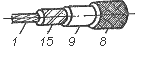
\includegraphics[width=0.2\textwidth]{76_MGSHV.png}
\caption{МГШВ}
\end{figure}

\begin{verse}
1 --- жила из медной луженой проволоки;\\
15 --- изоляция лентами из триацетатной пленки или пленки из полиэтилентерефталата;\\ 
8 --- оплетка из медной посеребренной проволоки;\\ 
9 --- изоляция из полихлорвинилового пластиката;\\
\end{verse}

МГТФ монтажный термостойкий фторопластовая изоляция. Провод МГТФ используется для монтажа радиоаппаратуры и других видов техники.Он широко применяется в судостроительстве, авиапромышленности.

\begin{figure}[H]
\centering
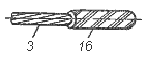
\includegraphics[width=0.2\textwidth]{76_MGTV.png}
\caption{МГТВ}
\end{figure}

\begin{verse}
3 --- жила из медных проволок;\\ 
16 --- изоляция лентами из фторопласта-4;\\
Э ---экранированный.\\
\end{verse}

МГВ --- многопроволочный  изолированный полихлорвинилом.

\begin{figure}[H]
\centering
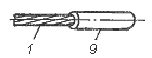
\includegraphics[width=0.2\textwidth]{76_MGV.png}
\caption{МГВ}
\end{figure}

\begin{verse}
1 --- жила из медной луженой проволоки;\\
9 --- изоляция из полихлорвинилового пластиката.\\ 
\end{verse}
Применение: Для фиксированного монтажа схем слаботочной радиоаппаратуры и электроприборов. Лаковая пленка изоляции эластична, малогорюча и обеспечивает высокую стойкость к воздействию тепла, холода и влаги.
\\ \\
МГШ --- многопроволочный изолированный оплеткой из шелка.

\begin{figure}[H]
\centering
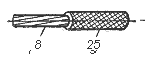
\includegraphics[width=0.2\textwidth]{76_MGSH.png}
\caption{МГШ}
\end{figure}

\begin{verse}
8 --- оплетка из медной посеребренной проволоки;\\ 
25 --- оплетка из полиамидного шелка.\\
\end{verse}
Применение: Для фиксированного монтажа схем слаботочной радиоаппаратуры.
\\ \\
МГШДЛ -/-/-/- лакированный;
МПМ --- многопроволочный изолированный полиэтиленом;
МШП --- однопроволочный изолированный обмоткой из шелка и полиэтиленом.

\begin{figure}[H]
\centering
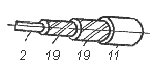
\includegraphics[width=0.2\textwidth]{76_MSHP.png}
\caption{МШП}
\end{figure}

\begin{verse}
2 --- жила из медной луженой проволоки;\\ 
11 --- изоляция из полиэтилена;\\ 
19 --- обмотка из шелка лавсан.\\
\end{verse}
Применение: Для фиксированного внутри- и межприборного монтажа.
\\ \\
ПМВ --- однопроволочный изолированный.

\begin{figure}[H]
\centering
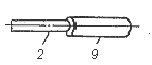
\includegraphics[width=0.2\textwidth]{76_PMV.png}
\caption{ПМВ}
\end{figure}

\begin{verse}
2 --- жила из медной луженой проволоки;\\ 
9 --- изоляция из полихлорвинилового пластиката.\\
\end{verse}
Применение: Для фиксированного монтажа слаботочной радиоаппаратуры.
\\ \\
ПВХ; ПМВГ --- многопроволочный с обмоткой из х/б пряжи
БПВЛ --- бортовой ПХВ изоляцией лакированный в х/б оплетке; ПВЛ --- провод высоковольтный в резиновой изоляции в лакированной х/б обмотке.

МСТП --- монтажный в обмотке из стекловолокна теплостойкий с полиэтиленовой изоляцией.
На качество паяных соединений оказывают существенное влияние не только технологические условия проведения процесса пайки, но и правильный выбор материала. Флюсы образуют  жидкую и газообразную защитные зоны, предохраняя поверхность пайки от окисления, растворяют и удаляют имеющийся пленки оксида и загрязнения с поверхностей улучшают смачивание металла припоем и растекание припоя за счет уменьшения силы поверхностного натяжения. Выбор флюса производится исходя из требований химической активности, которая должна быть наибольшей в диапазоне температур, определяемой температурой плавления и пайки. Он должен быстро и равномерно растекается по паяным материалам, хорошо приникать в зазоры и удалятся из них, резко вытесняется расплавленым припоем, быть термически стабильным, не выделять вредных газов, не вызывать коррозии паяных металлов и припоев. В зависимости от температурного интервала активные флюсы разделяются на низко- и высокотемпературные флюсы: 
\begin{verse}
Канифоль марок А,С.\\
ФКСп --- сосновая канифольная;\\ 
ФКЭт --- этиловый спирт 90;\%\\
ЛТИ120 --- сосновая канифольная 20-25\%.\\
\end{verse}

Припои различают низко и высокотемпературные. Граница раздела 400 \textcelsius. Высокотемпературные имеют высокую прочность и используются для пайки корпусных изделий, а также при использовании вторичной пайки. Используют: ПОС18(277 \textcelsius --- для не ответственных паек) ПОС40(235 \textcelsius), ПОС61 (190 \textcelsius) для ответственных паек, ПОС90(231 \textcelsius) пайка под гальванику, ПОСК50(145 \textcelsius) ответственные соединения керамики, серебра, стекла), сплав РОЗЕ (64 \textcelsius).

Флюс образуют газовую и жидкую фазы. При нагревании образуется зона повышенного давления, в которой не поступает кислород. Жидкая фаза: разрушает окисные пленки, уменьшает силы поверхностного натяжения.
Существуют: кислотные флюсы, бескислотные, антикоррозионные и активированные

% Вопрос 77 -----------------------------------------------------------------
\section{Волоконно-оптические линии связи (ВОЛС). Примеры использования.}

ВОЛС находят всё большее применение в устройствах передачи изображений, для обмена информацией между различными устройствами ЭВМ или отдельными машинами в вычислительных сетях, иерархических системах обработки информации.

По мнению специалистов ВОЛС займут доминирующее положение. Это связано:

\begin{enumerate} 
\item с малым поперечным сечением и малой массой волокон;
\item большой широкополостностью;
\item невосприимчивостью к внешним электромагнитным помехам- отсутствием внешних излучений;
\item отсутствием К.З.;
\item широким температурным диапазоном работы.
\end{enumerate}

Основу ВОЛС составляет световод или оптическое волокно. Схема прохождения сигнала поясняется следующим рисунком:

\begin{figure}[H]
\centering
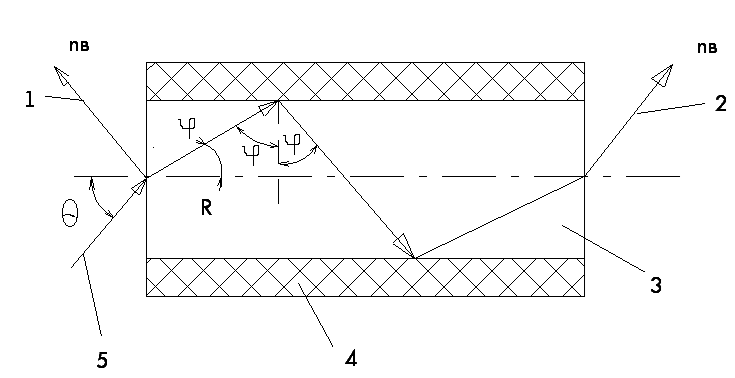
\includegraphics[width=0.6\textwidth]{77_opvol.png}
\caption{ВОЛС}
\end{figure}
\begin{enumerate} 
\item отраженный луч света
\item выходящий луч света
\item сердцевина
\item оболочка
\item падающий луч света
\end{enumerate} 

Луч света падающий под углом $\Theta$ на торец световода, проходит в его сердцевину и отражается под углом R от оболочки. Отражение происходит вследствие разности коэффициента отражения оболочки $n_{0}$ и сердцевины $n_{c}$. После многократного отражения луч света выходит из противоположного конца световода практически неизменным.

Показатели преломления сердцевины и оболочки определяют эффективность ввода излучения в световод. Чем больше разница, тем эффективнее световод. Неоправданно большая разница между показателями преломления сердцевины и оболочки ведет к увеличению дисперсии (расширения импульса). Затухание света в световод обусловлено поглощением и рассеиванием в материале сердцевины и потерям на излучение. Степень поглощения света материалом световода определяется его примесями, каждый вид которой обладает определенной полосой поглощения. Уширение импульса в световодах происходит из-за наличия в них: дисперсии материала, межмодовой дисперсии.
 
Межмодовая дисперсия --- следствие того, что свет введенный в световод под углом к оси, проходит более длинный путь, по сравнению со светом распространяющимся вдоль оси. Эта разница длин приводит к расплыванию входного импульса.

Дисперсия материала обуславливается нелинейной зависимостью показателя преломления материала от длины волны света. Изгибы световода приводят к потерям на излучение, которые сильно возрастают с уменьшением радиуса изгиба. Наименьший допустимый радиус кривизны ограничен фактической прочностью световодов.

Относительная деформация определяется:
\begin{eqnarray}
G_{s}=(((R+2r)/(R+r))-1)*100\%
\end{eqnarray}
\begin{verse}
где  r --- радиус оболочки световода, м;\\
R --- радиус изгиба световода, м\\
\end{verse}

Конструктивно световод состоит из сердцевины, покрытой несколькими слоями защитных материалов. Первичное покрытие (5…10 мкм), лаковая плёнка из ацетата целлюлозы, эпоксидной смолы, силикона, уретана и др., защищает материал сердцевины от внешних воздействий и увеличивает механическую прочность. Назначение последующих слоёв- устранение действующих поперечных сил и увеличение прочности на разрыв.

Отечественная промышленность выпускает большинство конструкций оптических кабелей, характеризующихся широким спектром параметров:

\begin{enumerate} 
\item $\varnothing$ наружный  4-8 мм
\item прочность на разрыв- 50-250 Н
\item коэффициент затухания 5-50 дб/км
\item погонная масса 10-50 кг/км
\item температура -40…+70 \textcelsius
\end{enumerate}
В качестве источника света --- светодиоды, лазерные диоды.

\begin{figure}[H]
\centering
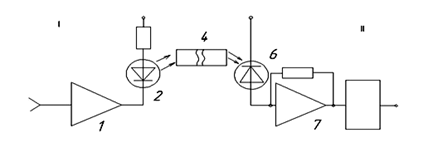
\includegraphics[width=0.6\textwidth]{77_sxema.png}
\caption{Схема ВОЛС}
\end{figure}

\begin{tabular}{llll}
I- передатчик &  1- возбудитель  & 4- оптический кабель & 7- усилитель \\ 
II- приёмник &  2- светодиод &  6- фотодиод  &  \\ 
\end{tabular} 

В ВОЛС со скоростью передачи информации до 50 Мбит/с следует использовать светодиоды, при более высоких скоростей- лазерные диоды. В случае необходимости включают регенерирующие устройства, обеспечивающие промежуточное усиление ослабленных сигналов и передачу усиленных сигналов в последующие участки ВОЛС.

Оптическое волокно используется телекоммуникационными компаниями для передачи телефонных сигналов, интернет-коммуникаций и сигналов кабельного телевидения. Из-за очень низкого ослабления и искажения сигнала, оптическое волокно имеет большие преимущества перед существующим медным проводом особенно на длинных расстояниях сохраняя высокие требования к передающей информации. Однако, развитие инфраструктуры в пределах городов было относительно трудным и отнимали много времени. Оптические волоконные системы были сложны и дороги при установке и в эксплуатации. Из-за этих трудностей, оптические волоконные системы в коммуникациях связи были прежде всего внедрены в районах с большими протяжённостями, где они используются обеспечивая передачу полного объёма нужной информации, компенсируя высокую стоимость.


% Вопрос 78 -----------------------------------------------------------------
\section{Эргономические требования к пультам, органам управления и сигнализации.}

Размещение органов управления должно подчиняться следующим общим правилам:

\begin{enumerate}
\item Количество и траектории рабочих движений должны быть сокращены до минимума;
\item Органы управления надо располагать так, чтобы правой рукой выполнять наиболее ответственные операции например, установку частоты, фокуса и т. п.;
\item Если орган управления находится рядом с индикатором, то ручка, управляемая правой рукой, должна находится правее и ниже, а ручка управляемая левой рукой, --- левее и ниже индикатора;
\item Последовательно используемые органы управления надо располагать на одной высоте слева направо или сверху вниз в вертикальных столбцах;
\item Основные органы управления целесообразно размещать в оптимальной зоне, аварийные --- в средней зоне досягаемости руки и второстепенные в зоне максимальной досягаемости.
\end{enumerate}

Взаимодействие человека с ЭВС осуществляется в основном через лицевую панель или пульт управления, на котором выделяют:

\begin{enumerate} 
\item средства отображения информации --- индик., ЭЛТ; 
\item органы управления --- тумблеры , регуляторы;
\item элементы коммутации --- ручки, фиксаторы; 
\item поясняющие надписи.
\end{enumerate}

При конструировании решают вопросы размещения на заданной площади всех составных частей, отвечающих требованиям эргономики, создание художественного образа изделия. Эргономические показатели можно разбить на группы: гигиенические, антропометрические, физиологические, психологические. 

Органы управления разделяют на элементы регулировки и элементы управления. Элементы регулировки --- переменные резисторы должны соответствовать схеме. Оперативность работы обеспечивается с помощью переключателей. Клавиши переключателей могут иметь различную форму и цвет. Рекомендуется для надежной установки кольца рабочую поверхность делать выгнутой. Диаметр кнопок --- не менее 12,5 мм. Перемещение кнопок --- на глубину 3…12 мм. Помимо механических кнопок могут использоваться сенсорные переключатели --- для них необходима визуальная индикация состояния.

Когда требуется четкое восприятие положения переключателя используют тумблеры. При переводе тумблера из одного положения в другое должен ощущается перепад сопротивлений упругости, а  при переключении --- щелчок. Также применяют галетные переключатели. Конструкция переносного пульта управления должна удовлетворять следующим требованиям:

\begin{enumerate}  
\item при разработке переносного пульта управления должны учитываться требования эргономики; 
\item должна быть обеспечена невозможность включения автоматического режима работы при использовании пульта в огражденном пространстве; 
\item на переносном пульте управления должен быть орган аварийного отключения; 
\item переносной пульт управления, предназначенный для включения перемещения промышленного робота (ПР) обслуживающим персоналом, находящимся в огражденном пространстве, должен быть снабжен устройством(ами) толчкового управления; 
\item система управления ПР должна быть сконструирована так, чтобы при управлении ПР с пульта все движения ПР осуществлялись только с этого пульта; 
\item все перемещения ПР, которые выполняются с пульта, должны осуществляться на скорости, не превышающей пониженную скорость. Пониженная скорость должна выбираться в зависимости от грузоподъемности ПР и схемы его расположения, однако пониженная скорость, измеренная на фланце крепления инструмента или зажима, должна быть не более 250 мм/с. 
\end{enumerate}

В тех случаях, когда требуется скорость выше, чем пониженная, например для проверки правильности программы, оператор должен включать этот режим, находясь за пределами огражденного пространства. Пока оператор остается в огражденном пространстве, движение ПР должно осуществляться только с помощью устройства толчкового управления.

\begin{figure}[H]
\centering
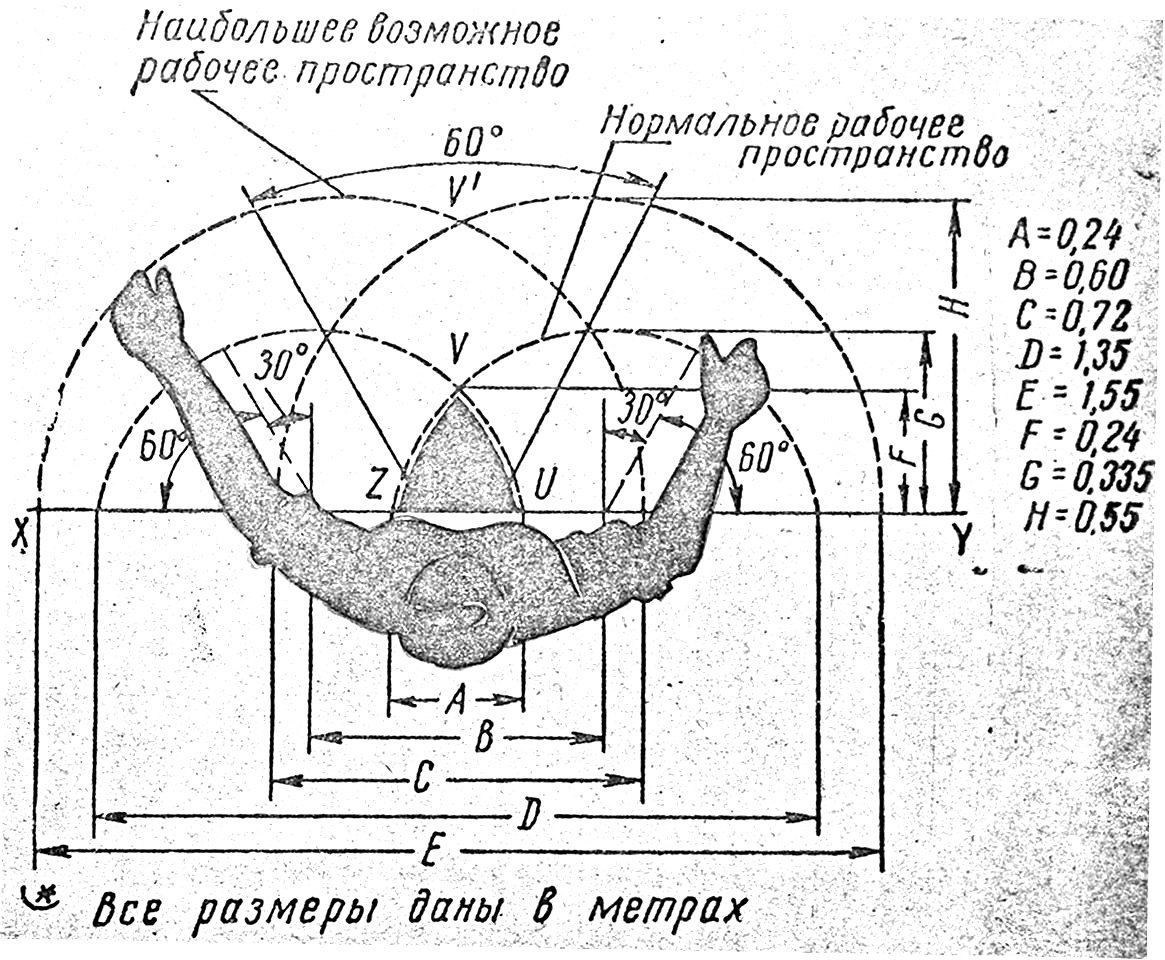
\includegraphics[width=0.6\textwidth]{78_operator.png}
\caption{Зона досягаемости оператора}
\end{figure}

% Вопрос 79 -----------------------------------------------------------------
\section{Эргономика конструирования лицевой панели прибора.}

Предпочтительными бывают следующие формы: фронтальная, трапецеидальная, полукруглая. Для всех существуют единые требования:

\begin{enumerate}
\item Передняя панель должна находиться перпендикулярно плоскости взгляда;
\item Органы управления должны в поле доступа оператора;
\item Предпочтительны ситуации, в которых доступ к органам управления осуществляется поворотом руки, кисти. \item Нежелательны ситуации, требующие поворота туловища;
\item Направление движения регулятора должно находиться в поле доступа человека-оператора;
\item Основой внешней конструкции любого устройства ЭВА является его ЛПУ.
\end{enumerate}

Методика конструирования ЛПУ заключается в следующей последовательности проведения необходимых работ:

\begin{enumerate}
\item Анализ исходных данных для проектирования;
\item Набор комплектующих элементов;
\item Структурирование ЛПУ;
\item Эргономическое обеспечение ЛПУ;
\item Композиционная отработка ЛПУ;
\item Цветовая проработка и выбор варианта декоративного решения , т.е. по существу; художественно-конструкторский анализ изделия ЭВА с ЛП.
\end{enumerate}

Изложенная последовательность разработки ЛПУ обусловлена тем , что эстетический фактор не является превалирующим для большинства типов ЭВА. Некоторое исключение составляет бытовая аппаратура , например калькуляторы. Поэтому эргономические требования занимают более высокое место по сравнению с эстетическими, так как они существенно влияют на быстродействие и безошибочность работы оператора , т.е. эксплуатационную надежность ЭВА. Поэтому порядок учета и приоритет требований должен быть однозначным. Поскольку ТЗ обычно составляет сам разработчик ЭВА , то ему необходимо согласовать с заказчиком ЭВА характеристики внешних условий и особенности работы оператора, часто этот момент , к сожалению , забывается при составлении ТЗ как заказчиком , так и самими разработчиком. В последствии эта недоработка вскрывается на этапе эксплуатации ЭВА.
Эргономические требования считаются граничными условиями, при которых в дальнейшем должен производится поиск выразительного художественного решения ( формы , композиции , цвета ).

АНАЛИЗ ИСХОДНЫХ ДАННЫХ ДЛЯ КОМПОНОВКИ ЛПУ:

В качестве исходных данных для разработки ЛПУ для инженера-конструктора ЭВА обычно выступают следующие:
\begin{enumerate}
\item Техническое задание на разработку устройства ЭВА с указанием характеристик внешних условий и особенностей работы оператора;
\item Схема электрическая принципиальная , разработанная инженером-схемотехником с указанием на ней элементов индикации , управления и коммутации;
\item Описанию порядка работы с устройством (алгоритм подготовки устройства к работе и работа с устройством).
\end{enumerate}
Это описание должно составляется инженером конструктором совместно со схемотехником. Компоновка лицевой панели начинается с формирования функциональных групп типа индикатор-регулятор-символ. Возможны три варианта их расположения: регулятор относительно индикатора слева, справа, снизу. Но при этом необходимо учитывать возможность работы оператора правой (в правой части панели) или левой рукой (в левой части панели). При воздействии на органы управления соответствующие индикаторы не должны перекрываться рукой. Надписи и символы располагаются над или между соответствующими регуляторами и индикаторами. При работе человека с РЭС основное количество информации к нему поступает через зрение. Способность человека зрительно воспринимать информацию характеризуется полем зрения обоих глаз, остротой зрения, фокусировкой, способность изменять чувствительность глаза в зависимости от уровня освещенности --- адаптацией, нацеливанием глаза в одну точку с помощью совместного действия глазных мышц и хрусталика, при переводе 
взгляда, цветным восприятием.

% Вопрос 80 -----------------------------------------------------------------
\section{Защита ЭС от воздействий радиации.}

Конструирование РЭА предусматривает выбор материалов и элементной базы, а также конструктивных решений, уменьшающих влияние радиации.
Ионизирующей радиацией – называется облучение, обладающее свойством проникать в толщу вещества и вызывать в нем ионизацию. Воздействие радиации на вещество зависит от вида радиации.
Воздействие гамма – лучей имеет объемный характер. Под влиянием гамма – излучения возникает сильная ионизация, явление фотопроводимости, люминесценция, химические реакции, повышение температуры, изменение анизотропных свойств кристаллических веществ. Облучение электронами ($\beta$ - излучение) носит поверхностный характер и вызывает ионизацию, вторичную эмиссию, небольшие изменения в решетке вещества, жесткое рентгеновское облучение. Воздействие $\alpha$ - частиц и осколков ядер можно практически не учитывать вследствие малой длины пробега и поверхностного характера.

Органические вещества весьма чувствительны к радиации. Воздействие приводит к преобразованию молекул, сопровождающемуся химическими реакциями, вызывающими необратимые изменения природы вещества и его механических свойств. Фенолформальдегид и метилметакрилат становятся хрупкими и деформируются. Полиэтилен и полистирол – вначале увеличивается сопротивление разрыву и твердость, а затем они становятся хрупкими. Большинство пластмасс темнеет и обесцвечивается. Пропитки и изоляционные масла портятся, как и оргматериалы.

На неорганические вещества (материалы) радиация воздействует меньше, чем на органические. 

При конструировании необходимо:

\begin{enumerate}
\item правильно подбирать и располагать элементы,
\item шире использовать керамические изоляторы в частях переключателей, разъемах, гнездах и т. д.,
\item применять стеклоткань и другие неорганические материалы для манжет, кабельной изоляции и др.,
\item применение элементов из неорганических материалов, слюдяных и керамических конденсаторов,
\item применять пленочные и металлопленочные сопротивления,
\item тщательно продумывать схему расположения, для уменьшения токов утечки и пробоя,
\item экранировать наиболее чувствительные элементы,
\item правильно выбирать материалы деталей конструкции,
\item правильно выбирать полупроводниковые приборы.
\end{enumerate}

Для защиты от $\gamma$ --- лучей хорошо экранируют, защищают --- свинец, уран, торий, висмут, вольфрам, золото, платина, ртуть и некоторые другие тяжелые материалы.

Для защиты от нейтронов применяют экраны из смеси легких и тяжелых элементов (бетон с повышенным содержанием воды), бороль (сплав карбида бора с алюминием), литий, бериллий, железо, медь, вольфрам, висмут.

\end{document}